% Developing a digital synthesizer in C++

\documentclass[12pt,twoside]{report}

\usepackage{listings}

\usepackage{color}

\usepackage{url}

\usepackage{graphicx}

\usepackage{newtxtext}

\usepackage[labelfont=bf]{caption}

\usepackage[a4paper,margin=1in]{geometry}

\usepackage{fancyhdr}

\usepackage{mathtools}

\usepackage{gensymb}

\usepackage{multicol}

\usepackage{multirow}

\usepackage{floatrow}

\usepackage{array}

\usepackage[toc,page]{appendix}

\usepackage{colortbl}

\setlength{\headheight}{15pt}

\begin{document}

\everymath{\displaystyle}

\fancyhf{}
%\renewcommand{\headrulewidth}{0pt}
\fancyhead[LO]{\leftmark}
\fancyhead[RE]{SECTION \rightmark}
\fancyhead[RO,LE]{\thepage}

\pagestyle{fancy}

\definecolor{custommagenta}{RGB}{230,70,165}
\definecolor{customgreen}{RGB}{30,210,100}
\definecolor{customgray}{gray}{0.5}

\lstset{
% Format settings
language=C++,
tabsize=4,
breakatwhitespace=true,
breaklines=true,
frame=leftline,
captionpos=b,
keepspaces=true,
showstringspaces=false,
numbers=left,
numberstyle=\scriptsize,
% Style settings
basicstyle=\ttfamily\scriptsize,
keywordstyle=\color{custommagenta}\ttfamily,
stringstyle=\color{customgreen}\ttfamily,
commentstyle=\color{customgray}\ttfamily,
morecomment=[l][\color{red}]{\#}
}

% Macro for source code inclusion. Moves to main
% directory then takes the further path as argument
\newcommand{\code}[2][1]{\lstinputlisting[firstnumber=#1]{code/#2}}

\newcommand{\citebs}[1]{(Mitchell, 2008, p. #1)}

\newcommand{\citedsp}[1]{(Smith, 1999, p. #1)}

\newcommand{\sidecap}[3]{\floatbox[{\capbeside\thisfloatsetup{capbesideposition={right,center}}}]{table}[\FBwidth]{\caption{#1} \label{#2}}{#3}}

\newfloatcommand{capbtabbox}{table}[][\FBwidth]

\title{Developing a Digital Synthesizer in C++}

\author{
Peter Goldsborough\\
\texttt{petergoldsborough@hotmail.com}
}

\date{\today}

\maketitle

\tableofcontents

\chapter{Sound in the Digital Realm}

\section{What is a Music Synthesizer?}



\section{From Analog to Digital}

Our everyday experience of sound is an entirely analog one. When a physical     object emits or reflects a sound wave into space and towards our ears, the signal produced consists of an infinite set of values, spaced apart in infinitesimal intervals. Due to the fact that such a signal has an amplitude value at every single point in time, it is called a continuous signal. \citedsp{11} Figure \ref{fig:cont} displays the continuous representation of a sine wave.

\begin{figure}[h!]

  \centering

  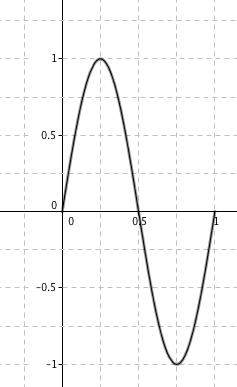
\includegraphics[scale=0.5]{img/cont}

  \caption{The continuous representation of a typical sine wave. In this case, both the signal's frequency $f$ as well as the maximum elongation from the equilibrium $a$ are equal to $1$. }

  \label{fig:cont}

\end{figure}

\pagebreak

\noindent While continuous signals and the idea of an infinite, uncountable set of values are easy to model in mathematics and physics --- the analog world, computers --- in the digital world --- effectively have no means by which to represent something that is infinite, since computer memory is a finite resource. Therefore, signals in the digital domain are discrete, meaning they are composed of periodic \emph{samples}. A sample is a discrete recording of a continuous signal's amplitude, taken in a constant time interval \citebs{16}. The process by which a continuous signal is converted to a discrete signal is called \emph{quantization}, \emph{digitization} or simply \emph{analog-to-digital-conversion} \citedsp{35-36} \citebs{16}. Quantization essentially converts an analog function of amplitude to a digital function of location in computer memory over time (Burk, Polansky, Repetto, Roberts and Rockmore, 2011, Section 2.1). The reverse process of converting discrete samples to a continuous signal is called \emph{digital-to-analog-conversion} \citebs{17}. Figure \ref{fig:disc} shows the discrete representation of a sine wave, the same signal that was previously shown as a continuous signal in Figure \ref{fig:cont}.

\begin{figure}[h!]

  \centering

  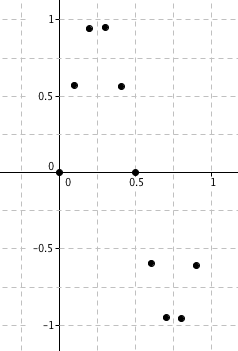
\includegraphics[scale=0.5]{img/disc}

  \caption{The discrete representation of a typical sine wave.}

  \label{fig:disc}

\end{figure}

\section{Sample Rate}

The sample rate (often referred to as sampling rate or sampling frequency), commonly denoted by $f_{s}$, is the rate at which samples of a continuous signal are taken. The value of the sample rate is given in Hertz (Hz) or samples-per-second. Common values for audio sampling rates are 44.1 kHz, a frequency originally chosen by Sony in 1979 that is still used for Compact Discs, and 48 kHz, the standard audio sampling rate used today \citebs{18} (Colletti, 2013). The reciprocal of the sample rate yields the sampling interval, denoted by $T_{s}$ and measured in seconds, which is the time period after which a single sample is taken from a continuous signal:\begin{center} $T_{s} = \frac{1}{f_{s}}$ \end{center} The reciprocal of the sample interval again yields the sampling rate: \begin{center} $f_{s} = \frac{1}{T_{s}}$ \end{center}

\section{Nyquist Limit}

The sample rate determines the range of frequencies that can be represented by a digital sound system, as only frequencies that are less than or equal to one half of the sampling rate, where it is possible to take at least one sample above the equilibrium and at least one sample below the equilibrium for every cycle \citebs{18}, can be "properly sampled". To sample a signal "properly" means to be able to "reconstruct" a continuous signal, given a set of discrete samples, "exactly", i.e. without any \emph{quantization errors}. The value of one half of the sample rate is called the \emph{Nyquist frequency} or \emph{Nyquist limit}, named after Harry Nyquist, who first described the Nyquist limit and associated phenomena together with Claude Shannon in the 1940s, stating that "a continuous signal can be properly sampled, only if it does not contain frequency components above one half the sampling rate" \citedsp{40}. Any frequencies above the Nyquist limit lead to \emph{aliasing}, which is discussed in the next section.\\

\noindent Given the definition of the Nyquist limit and considering the fact that the limit of human hearing is approximately 20 kHz (Cutnell \& Johnson, 1998, p. 466), the reason for which the two most common audio sample rates are 40 kHz and above is clear: they were chosen to allow the "proper" representation of the entire audio frequency range, since a sample rate of 40 kHz meets the Nyquist requirement of a sample rate at least twice the maximum frequency component of the signal to be sampled (the Nyquist limit), in this case ca. 20 Khz.

\section{Aliasing}

When a signal's frequency exceeds the Nyquist limit, it is said to produce an \emph{alias}, a new signal with a different frequency that is indistinguishable from the original signal when sampled. This is due to the fact that a signal with a frequency component above the Nyquist limit no longer has one sample taken above and one below the zero level for each cycle, but at arbitrary points of the original signal, which, when reconstructed, yield an entirely different signal. For example, if the sinusoid depicted in Figure \ref{fig:orig}, with a frequency of 4 Hz, is sampled at a sample rate of 5 samples per second, shown in Figure \ref{fig:sampled} meaning the frequency of the continuous signal is higher than the Nyquist limit (here 2.5 Hz), the reconstructed signal, approximated in Figure \ref{fig:approx}, will look completely different from the original sinusoid. "This phenomenon of [signals] changing frequency during sampling is called aliasing, [...] an example of improper sampling" \citedsp{40}.

\begin{figure}[b!]

  \centering

  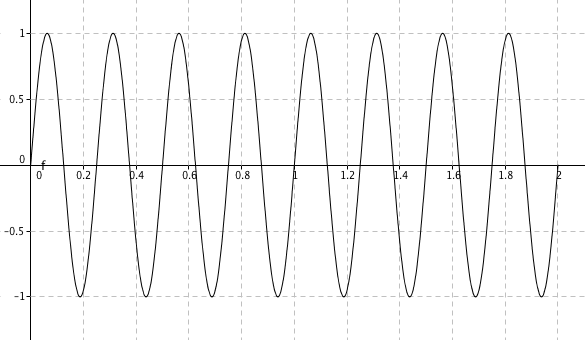
\includegraphics[scale=0.5]{img/orig}

  \caption{A sinusoid with a frequency of 4 Hz.}

  \label{fig:orig}

\end{figure}

\begin{figure}

  \centering

  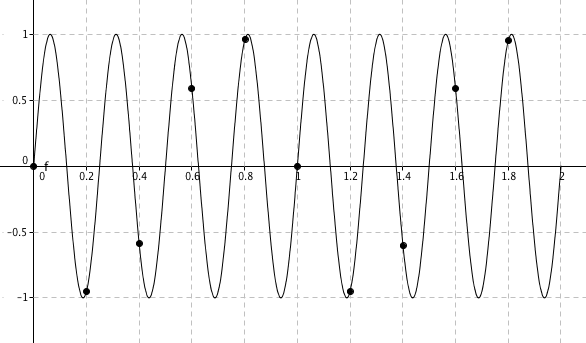
\includegraphics[scale=0.5]{img/sampled}

  \caption{A sinusoid with a frequency of 4 Hz, sampled at a sample rate of 5 Hz. According to the Nyquist Theorem, this signal is sampled improperly, as the frequency of the continuous signal is not less than or equal to one half of the sample rate, in this case 2.5 Hz. }

  \label{fig:sampled}

\end{figure}

\begin{figure}

  \centering

  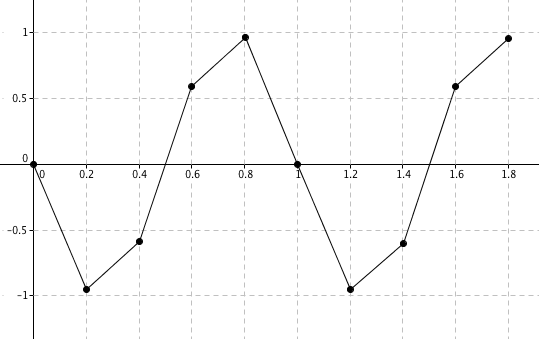
\includegraphics[scale=0.5]{img/approx}

  \caption{An approximated representation of the signal created from the sampling process shown in Figure \ref{fig:sampled}. Visually as well as acoustically, the new signal is completely different from the original signal. However, in terms of sampling, they are indistinguishable from each other due to improper sampling. These signals are said to be \emph{aliases} of each other.}

  \label{fig:approx}

\end{figure}

\section{Overflow}

Another interesting property of digital sound, which is not encountered in the analog world, is that it can overflow. When we attempt to increase the loudness of something in the analog world, e.g. by hitting a drum more intensely, the expected result is a louder sound. In the digital realm however, it may occur that attempting to increase a signal's amplitude does not result in an increased loudness, but in distortion. The cause of this phenomenon lies in the way digital audio is stored. Since computer memory is a finite resource, each sample has a dedicated portion of computer memory allocated to it. For example, the Waveform Audio File Format (WAVE), a common computer file format for audio data, stores each sample of an audio track as a 16-bit signed integer. A 16-bit signed integer gives a possible range of $-2^{16-1}$ to $2^{16-1}$ ($16-1$ because the most significant bit is used as the sign bit in two's complement representation). This means that a signal with an amplitude of 1 will be stored as 32767, an amplitude of 0.5 as 16384, an amplitude of -1 as -32768 and so on. If one tries to increase the amplitude of a signal whose value has already saturated the available range and space allocated to it, in this case 32767 on the positive end and -32768 on the negative end, the result is that the integer with which the sample is stored \emph{overflows}. Because WAVE files (and many other storage media) store samples as \emph{signed} integers, overflow always results in a change of sign:

$$32767_{10} = 0111111111111111_{2}$$
$$0111111111111111_{2} + 1 = 1000000000000000_{2} = -32768_{10}$$
$$1000000000000000_{2} - 1 = 0111111111111111_{2} = 32767_{10}$$

A visualization of the result of increasing the amplitude of a signal with a saturated value (an amplitude of 1), shown in Figure \ref{fig:no-over}, is given in Figure \ref{fig:over}.

\begin{figure}[h!]
  \centering
  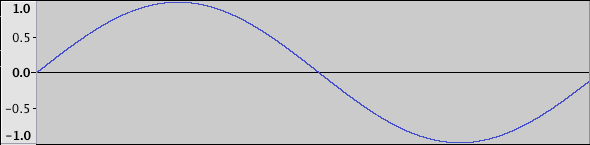
\includegraphics[scale=0.5]{img/no-over}
  \caption{A typical sinusoidal signal with an amplitude of 1. The integer range provided by the allocated memory for the top-most sample is saturated, meaning it is equal to $32767_{10}$ or $0111111111111111_{2}$.}
  \label{fig:no-over}
\end{figure}

\begin{figure}[h!]
  \centering
  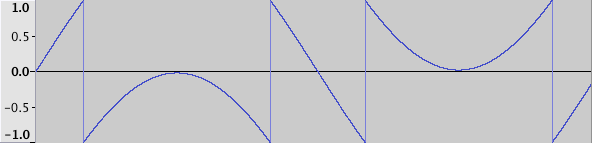
\includegraphics[scale=0.5]{img/over}
  \caption{What happens when the amplitude of the signal from Figure \ref{fig:no-over} is increased by a factor of 2. Multiple samples have overflowed and thus changed their sign. Because of the way two's-complement representation is implemented, the signal continues it's path as if no overflow had ever occurred. The only difference being, of course, that the sign has changed mid-way. }
  \label{fig:over}
\end{figure}

\chapter{Generating Sound}

The following sections will outline how digital sound can be generated in theory and implemented in practice, using the C++ programming language.

\section{Simple Waveforms}

The simplest possible waveform is the sine wave. As a function of time, it can be mathematically represented by Equation \ref{eq:sine}, where $A$ is the maximum amplitude of the signal, $f$ the frequency in Hertz and $\phi$ an initial phase offset in radians:

\begin{equation}
  f_{s}(t) = A \sin(2 \pi  f t + \phi)
  \label{eq:sine}
\end{equation}

A computer program to compute the values of a sine wave with a variable duration, implemented in C++, is shown in Listing \ref{code:sine}. Another waveform similar to the sine wave is the cosine wave, which differs only in a phase offset of 90\degree or $\frac{\pi}{2}$ radians:\\
\begin{equation}
  f_{c}(t) = A \cos(2 \pi  f t + \phi) = A \sin(2 \pi f t + \phi + \frac{\pi}{2})
  \label{eq:cosine}
\end{equation}\\
Therefore, the program from Listing \ref{code:sine} could be modified to compute a cosine wave by changing line 22 from:\\

\begin{lstlisting}[firstnumber=22]
  double phase = 0;
\end{lstlisting}
to
\begin{lstlisting}[firstnumber=22]
  double phase = pi/2.0;
\end{lstlisting}

\section{Complex Waveforms}

Now that the process of creating simple sine and cosine waves has been discussed, the generation of more complex waveforms can be examined. Generally, there are two methods by which complex waveforms can be created in a digital synthesis system: mathematical calculation or additive synthesis.

\subsection{Mathematical Calculation of Complex Waveforms}

In the first case --- mathematical calculation, waveforms are computed according to certain mathematical formulae and thus yield \emph{perfect} or \emph{exact} waveforms, such as a square wave that is equal to the maximum amplitude exactly one half of a period and equal to the minimum amplitude for the rest of the period. While these waveforms produce a very crisp and clear sound, they are rarely found in nature due to their degree of perfection and are consequently rather undesirable for a music synthesizer. Nevertheless, they are considerably useful for modulating other signals, as tiny acoustical imperfections such as those found in additively synthesized waveforms can result in unwanted distortion which is not encountered when using mathematically calculated waveforms. Therefore, exact waveforms are the best choice for modulation sources such as Low Frequency Oscillators (LFOs), which are discussed in later chapters. \citebs{71}\\\\
The following paragraphs will analyze how four of the most common waveforms found in digital synthesizers, the square, the sawtooth, the ramp and the triangle wave, can be generated via mathematical calculation.\\\\
\emph{Note: There have found to be disparities in literature over which waveform is a sawtooth and which a ramp wave. This thesis will consider a sawtooth wave as descending from maximum to minimum amplitude with time and a ramp wave as ascending from minimum to maximum amplitude with time.}

\subsubsection{Square Waves}

Ideally, a square wave is equal to its maximum amplitude for exactly one half of a period and equal to its minimum amplitude for the other half of the same period. A single period of a square wave can be calculated as shown in Equation \ref{eq:dsquare1}, where the independent variable $t$ as well as the period $T$ can be either in samples or in seconds. A mathematical Equation for a full, periodic square wave function is given by Equation \ref{eq:dsquare2}, where $t$ is time in seconds and the frequency $f$ in Hertz. An equivalent C++ computer program is shown in Table \ref{code:dsquare}.

\begin{multicols}{2}

  \begin{equation}
    f(t) =
    \begin{cases}
      1,& \text{if } 0 \leq t < \frac{T}{2}\\
      -1,& \text{if } \frac{T}{2} \leq t < T
    \end{cases}
    \label{eq:dsquare1}
  \end{equation}

  \begin{equation}
    f(t) =
    \begin{cases}
      1,& \text{if } \sin(2 \pi f t) > 0\\
      -1,& \text{otherwise}
    \end{cases}
    \label{eq:dsquare2}
  \end{equation}

\end{multicols}

\begin{table}
  \sidecap{C++ code to generate and return one period of a square wave, where \texttt{period} is the period duration in samples. Note that this function increments in sample time, measured in seconds, rather than actual samples. This prevents a one-sample quantization error at the mid-point, since time can always be halved whereas a sample is a fixed entity and cannot be broken down any further.}{code:dsquare}{\code{dsquare.cpp}}
\end{table}

\subsubsection{Sawtooth Waves}

An ideal sawtooth wave descends from its maximum amplitude to its minimum amplitude linearly before jumping back to the maximum amplitude at the beginning of the next period. A mathematical Equation for a single period of such a sawtooth wave function, calculated directly from the phase, is given by Equation \ref{eq:dsaw1} \citebs{68}. Alternatively, the function can depend on time or on samples, as shown by Equation \ref{eq:dsaw2}, where $T$ is the period. A computer program to compute one period of a sawtooth wave is given in Table \ref{code:dsaw}.

\begin{multicols}{2}

    \begin{equation}
      f(\phi) =
      \begin{cases}
        -\frac{\phi}{\pi} + 1,& \text{if } 0 \leq \phi < 2 \pi
      \end{cases}
      \label{eq:dsaw1}
    \end{equation}

    \begin{equation}
      f(t) =
      \begin{cases}
        -\frac{2t}{T} + 1,& \text{if } 0 \leq t < 1
      \end{cases}
      \label{eq:dsaw2}
    \end{equation}

\end{multicols}

\begin{table}
  \sidecap{C++ code to generate one period of a sawtooth wave function, where \texttt{period} is the period duration in samples.}{code:dsaw}{\code{dsaw.cpp}}
\end{table}

\subsubsection{Ramp Waves}

A ramp wave is, quite simply, an inverted sawtooth wave. It ascends from its minimum amplitude to its maximum amplitude linearly, after which it jumps back down to the minimum amplitude. Consequently, Equation  \ref{eq:dramp1} and \ref{eq:dramp2} differ from sawtooth Equation  \ref{eq:dsaw1} and \ref{eq:dsaw2} only in their sign and offset. The equivalent C++ implementation shown in Table \ref{code:dramp} also reflects these differences.

\begin{multicols}{2}

  \begin{equation}
    f(\phi) =
    \begin{cases}
      \frac{\phi}{\pi} - 1,& \text{if } 0 \leq \phi < 2 \pi
    \end{cases}
    \label{eq:dramp1}
  \end{equation}

  \begin{equation}
    f(t) =
    \begin{cases}
      \frac{2t}{T} - 1,& \text{if } 0 \leq t < 1
    \end{cases}
    \label{eq:dramp2}
  \end{equation}

\end{multicols}

\begin{table}
  \sidecap{C++ ramp wave generator. This code differs from the program shown in Table \ref{code:dsaw} solely in the amplitude offset (-1 instead of 1) and the increment, which is now positive. }{code:dramp}{\code{dramp.cpp}}
\end{table}

\pagebreak

\subsubsection{Triangle waves}

A triangle wave can be seen as a combination of a ramp wave and a sawtooth wave, or as a linear, "edgy", sine wave. It increments from its minimum amplitude to its maximum amplitude linearly one half of a period and decrements back to the minimum during the other half. Simply put, "[a] triangle wave is a linear increment or decrement that switches direction every $\pi$ radians" \citebs{69}. A mathematical definition for one period of a triangle wave is given by Equation  \ref{eq:dtri1}, where $\phi$ is the phase in radians. If $\phi$ is kept in the range of $[-\pi;\pi]$ rather than the usual range of $[0;2 \pi]$, the subtraction of $\pi$ can be eliminated, yielding Equation  \ref{eq:dtri2}. If the dependent variable is time, in seconds, or samples, Equation  \ref{eq:dtri3} can be used for a range of $[0;T]$, where $T$ is the period, and Equation  \ref{eq:dtri4} for a range of $[-\frac{T}{2};\frac{T}{2}]$. A C++ implementation is shown in Table \ref{code:dtri}.

\begin{multicols}{2}

  \begin{equation}
    f(\phi) =
    \begin{cases}
      1 - \frac{2 |\phi - \pi|}{\pi},& \text{if } 0 \leq \phi < 2 \pi
    \end{cases}
    \label{eq:dtri1}
  \end{equation}

  \begin{equation}
    f(\phi) =
    \begin{cases}
      1 - \frac{2 |\phi|}{\pi},& \text{if } -\pi \leq \phi < \pi
    \end{cases}
    \label{eq:dtri2}
  \end{equation}

\end{multicols}

\begin{multicols}{2}

  \begin{equation}
    f(t) =
    \begin{cases}
      1 - \frac{4 |t - \frac{T}{2}|}{T},& \text{if } 0 \leq t < 1
    \end{cases}
    \label{eq:dtri3}
  \end{equation}

  \begin{equation}
    f(t) =
    \begin{cases}
      1 - \frac{4 |t|}{T},& \text{if } -\frac{T}{2} \leq t < \frac{T}{2}
    \end{cases}
    \label{eq:dtri4}
  \end{equation}

\end{multicols}

\begin{table}
  \sidecap{C++ program to compute one period of a triangle wave.}{code:dtri}{\code{dtri.cpp}}
\end{table}

\subsection{Additive Synthesis}

The second method of generating complex waveforms, additive synthesis, produces waveforms that, despite not being mathematically perfect, are closer to the waveforms found naturally. This method involves the summation of a theoretically infinite, practically finite set of sine and/or cosine waves with varying parameters and is often called Fourier Synthesis, after the 18th century French scientist, Joseph Fourier, who first described the process and associated phenomena of summing sine and cosine waves to produce complex waveforms. This calculation of a complex, periodic waveform from a sum of sine and cosine functions is also called a Fourier Transform or a Fourier Series, both part of the Fourier Theorem. In a Fourier Series, a single sine/cosine component is either called a harmonic, an overtone or a partial. All three name the same idea of a waveform with a frequency that is an \emph{integer multiple} of some fundamental pitch or frequency. \citebs{64} Throughout this thesis the term \emph{partial} will be preferred. \\\\Equation 2.13 gives the general definition of a discrete Fourier Transform. Equation 2.14 shows a simplified version of Equation 2.13. Table \ref{code:partial} presents a C++ struct to represent a single partial and Listing \ref{code:add} a piece of C++ code to compute one period of any Fourier Series.

\begin{figure}[h!]
  $f(t) = \frac{a_{0}}{2} + \sum\limits_{n=1}^\infty (a_{n} \cos(\omega n t) = b_{n} \sin(\omega n t))$
  \caption*{\textbf{Equation 2.13: }Formula to calculate an infinite Fourier series, where $\frac{a_{n}}{2}$ is the center amplitude, $a_{n}$ and $b_{n}$ the partial amplitudes and $\omega$ the angular frequency, which is equal to $2 \pi f$.}
  \label{fig:fourier1}
\end{figure}

\begin{figure}[h!]
  $f(t) = \sum\limits_{n=1}^N a_{n} \sin(\omega n t + \phi_{n})$
  \caption*{\textbf{Equation 2.14:} Simplificiation of Equation 2.13. Note the change from a computationally impossible infinite series to a more practical finite series. Because a cosine wave is a sine wave shifted by 90\degree or $\frac{\pi}{2}$ radians, the $\cos$ function can be eliminated and replaced by an appropiate $\sin$ function with a phase shift $\phi_{n}$.}
  \label{fig:fourier2}
\end{figure}

\begin{table}
  \sidecap{C++ code to represent a single partial in a Fourier Series.}{code:partial} {\code{partial.cpp}}
\end{table}

\noindent The following paragraphs will examine how the four waveforms presented in Section 2.2.1, the square, the sawtooth, the ramp and the triangle wave, can be synthesized additively.

\subsubsection{Square Waves}

When speaking of additive synthesis, a square wave is the result of summing all odd-numbered partials (3rd, 5th, 7th etc.) at a respective amplitude equal to the reciprocal of their partial number ($\frac{1}{3}$, $\frac{1}{5}$, $\frac{1}{7}$ etc.). The amplitude of each partial must decrease with increasing partial numbers to prevent amplitude overflow. A mathematical equation for such a square wave with $N$ partials is given by Equation \ref{eq:asquare}, where $2n - 1$ makes the series use only odd partials. A good maximum number of partials $N$ for near-perfect but still naturally sounding waveforms is 64, a value determined empirically. Higher numbers have not been found to produce significant improvements in sound quality. Table \ref{code:asquare} displays the C++ code needed to produce one period of a square wave in conjuction with the \texttt{additive} function from Tables \ref{code:add1} and \ref{code:add2}. Figure \ref{fig:square} shows the result of summing 2, 4, 8, 16, 32 and finally 64 partials.

\begin{equation}
  f(t) = \sum\limits_{n=1}^N \frac{1}{2n -1} \sin(\omega (2n - 1) t)
  \label{eq:asquare}
\end{equation}

\begin{figure}

  \TopFloatBoxes

  \begin{floatrow}

    \ffigbox{\caption{Square waves with 2, 4, 8, 16,\\ 32 and 64 partials.} \label{fig:square}}{ 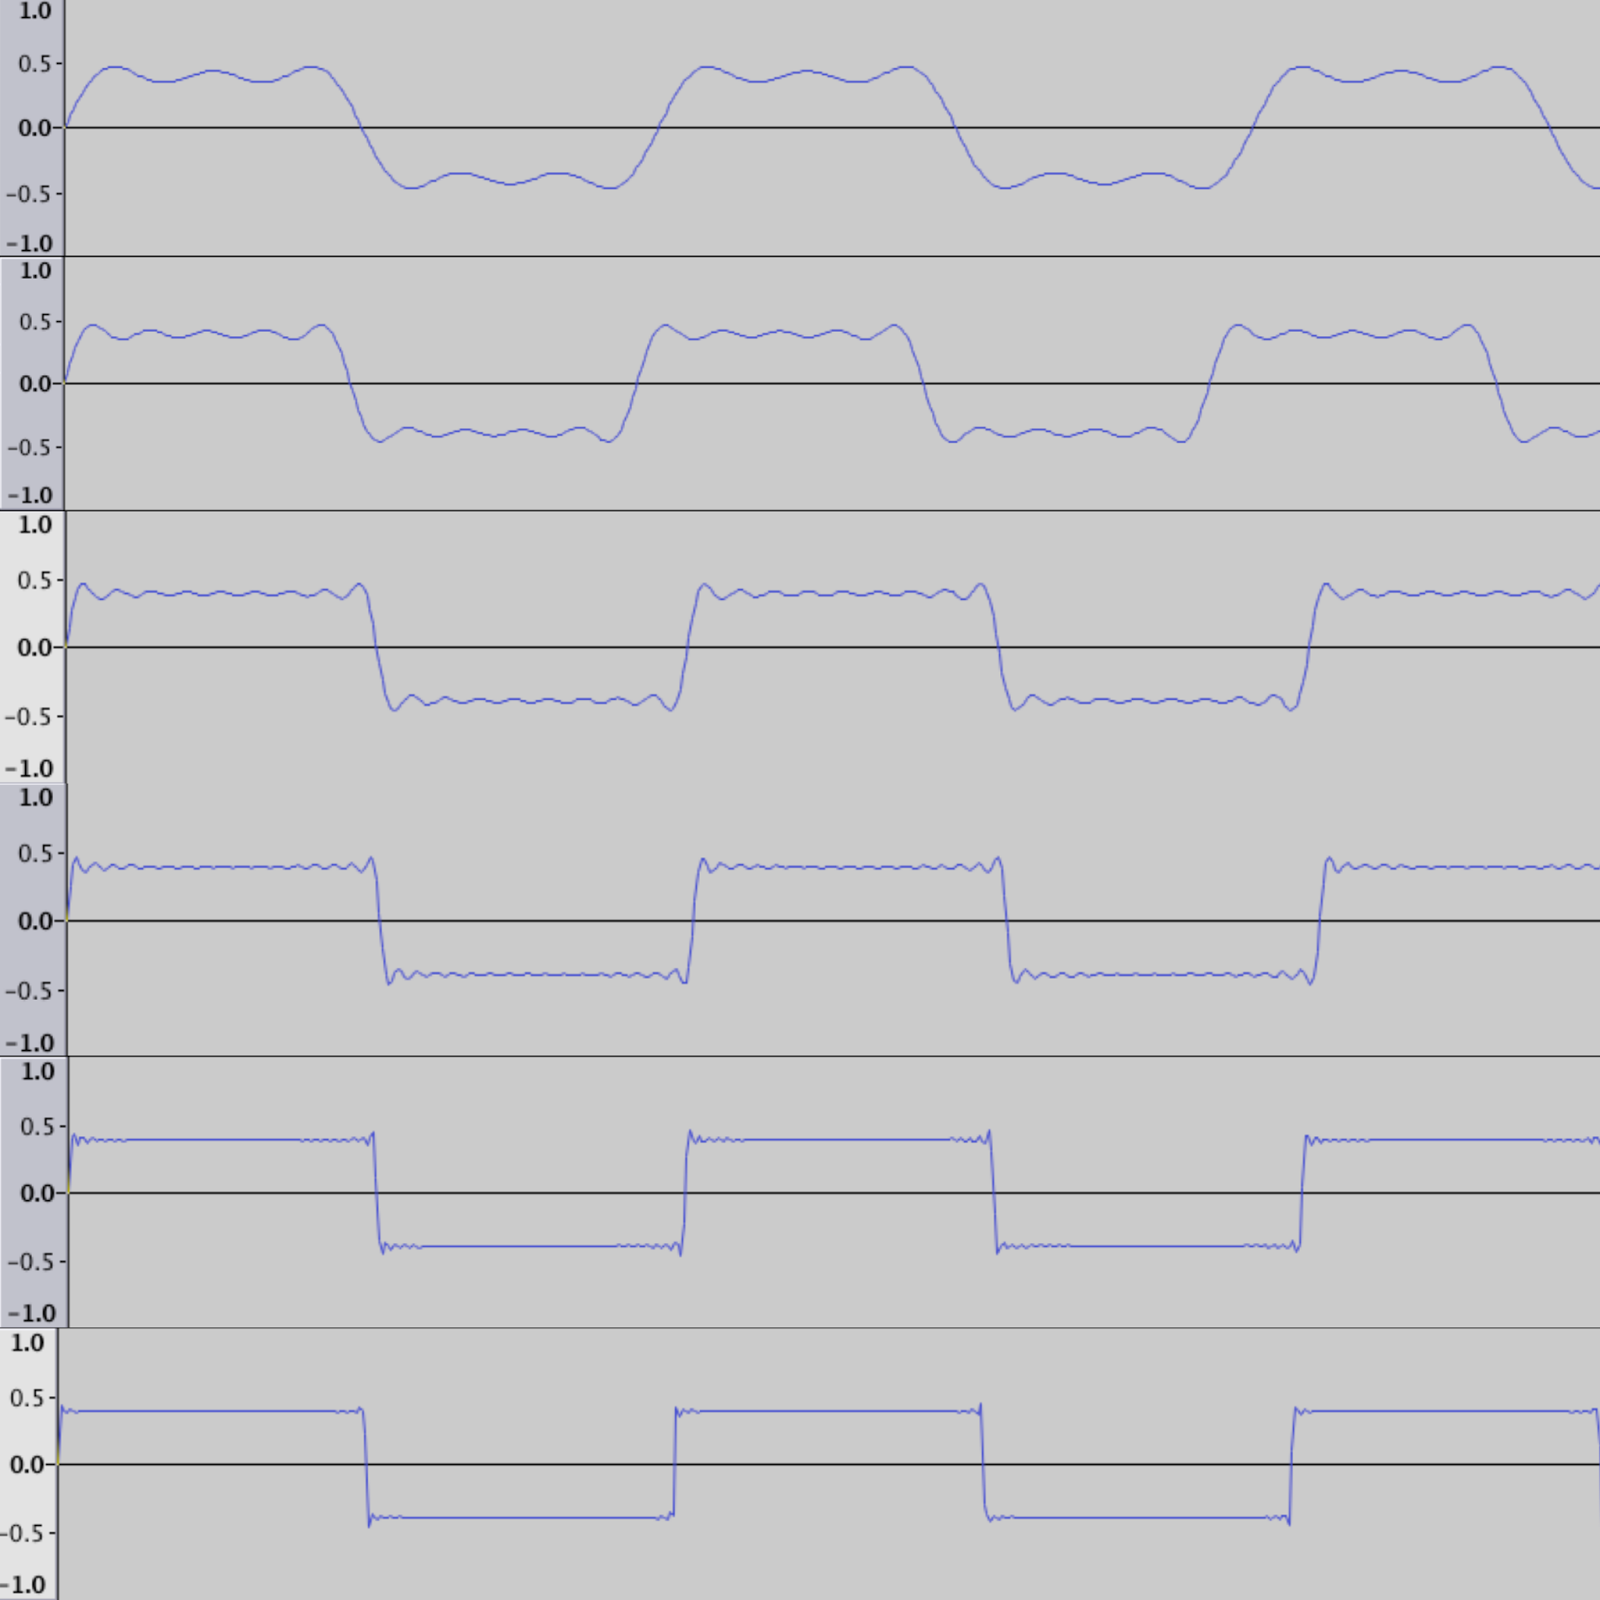
\includegraphics[scale=0.12]{img/square}}

    \ttabbox{\caption{C++ code for a square wave with 64 partials.} \label{code:asquare}}{\code{asquare.cpp}}

  \end{floatrow}

\end{figure}

\pagebreak

\subsubsection{Sawtooth Waves}

A sawtooth wave is slightly simpler to create through additive synthesis, as it requires the summation of every partial rather than only the odd-numbered ones. The respective amplitude is again the reciprocal of the partial number. Equation \ref{eq:asaw} gives a mathematical definition for a sawtooth wave, Figure \ref{fig:saw} displays sawtooth functions with various partial numbers and Table \ref{code:asaw} shows C++ code to generate such functions.

\begin{equation}
  f(t) = \sum\limits_{n=1}^N \frac{1}{n} \sin(\omega n t)
  \label{eq:asaw}
\end{equation}

\begin{figure}[h!]

  \TopFloatBoxes

  \begin{floatrow}

    \ffigbox{\caption{Sawtooth waves with 2, 4, 8,\\ 16, 32 and 64 partials.} \label{fig:saw}}{ 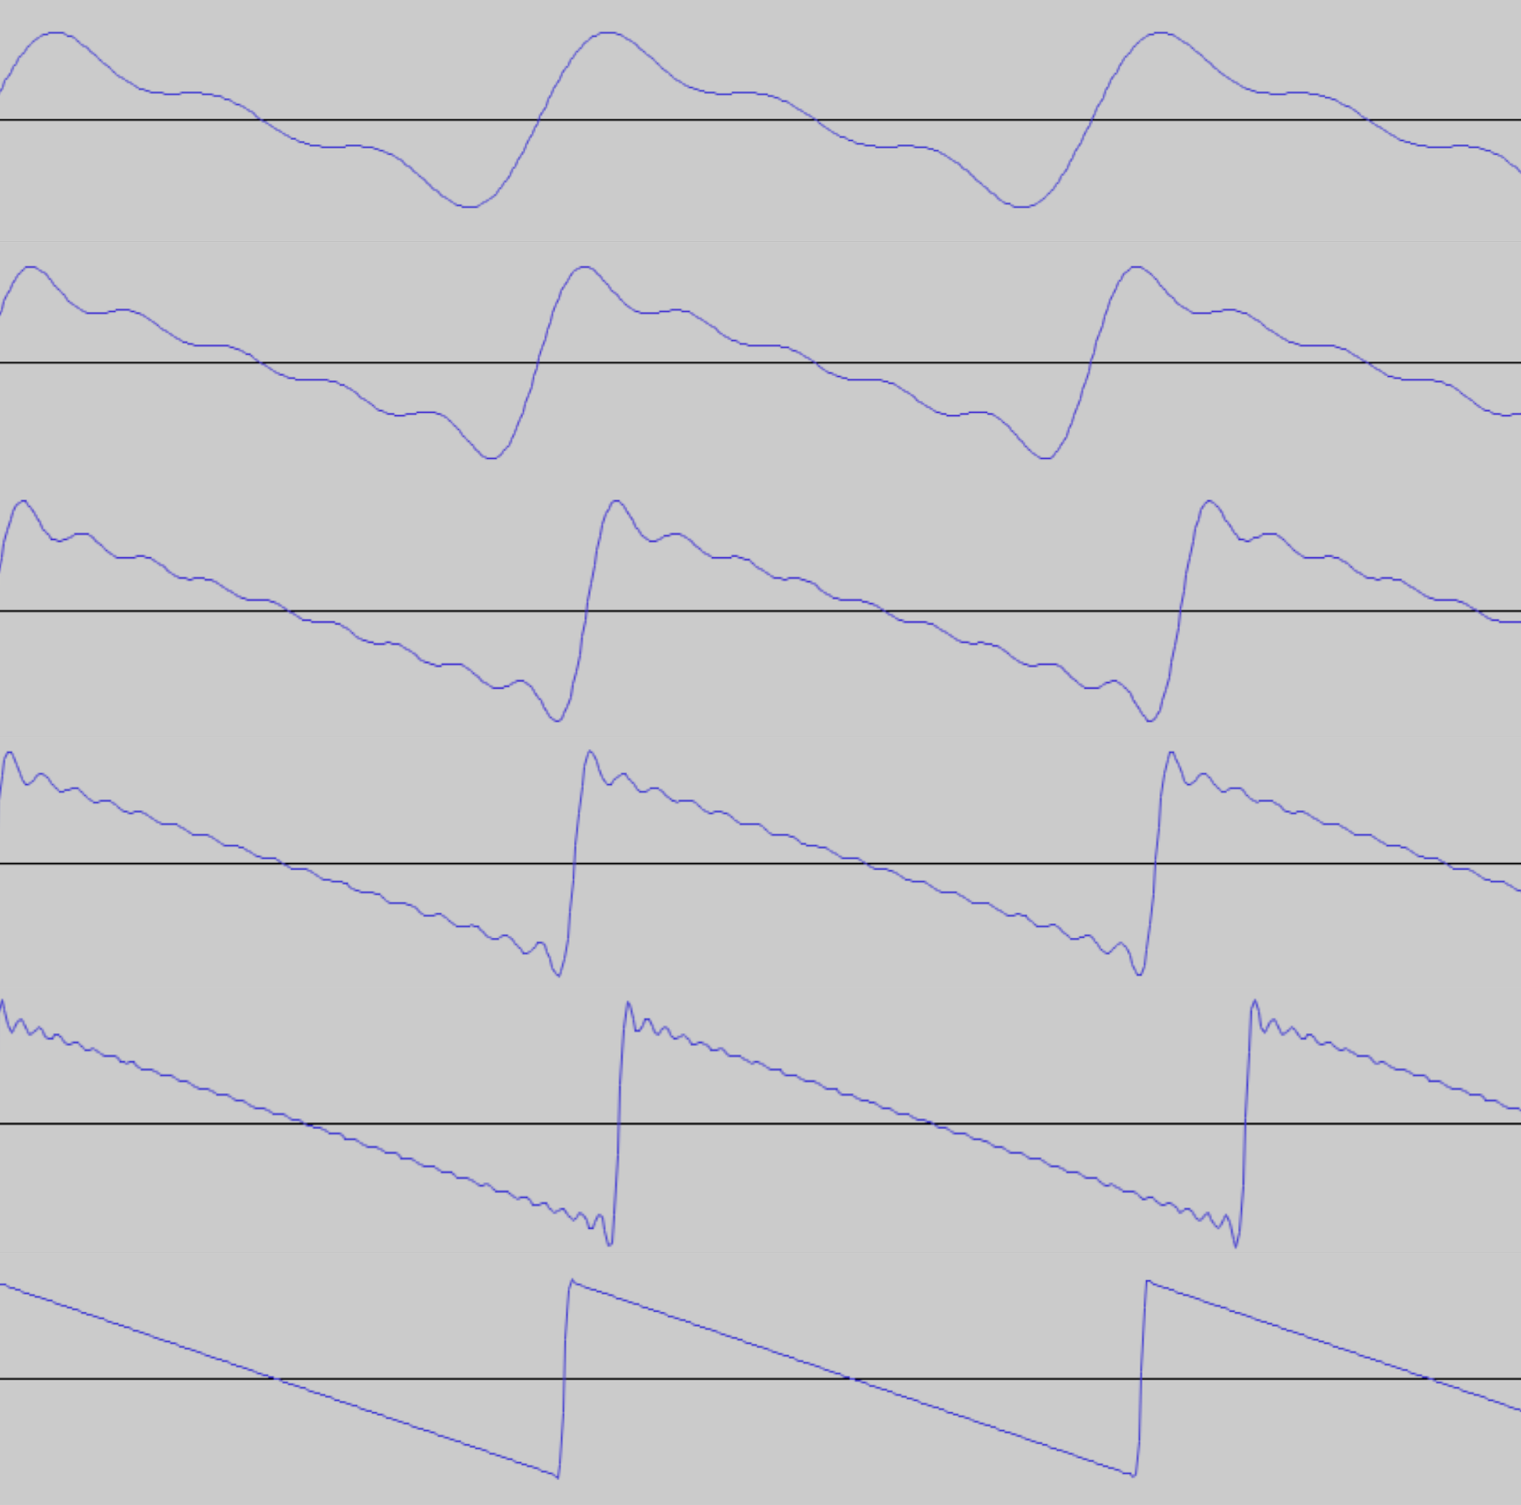
\includegraphics[scale=0.12]{img/saw}}

    \ttabbox{\caption{C++ code for a sawtooth wave with 64 partials.} \label{code:asaw}}{\code{asaw.cpp}}

  \end{floatrow}

\end{figure}

\pagebreak

\subsubsection{Ramp Waves}

Ramp waves are essentially the inverse of sawtooth waves. Therefore, we can simply sum sinusoids as we did for a sawtooth function but change the sign of each partial's amplitude to negative instead of positive. Equation \ref{eq:aramp} gives the mathematical definition, Figure \ref{fig:ramp} displays a set of ramp waveforms with different partial numbers and Table \ref{code:aramp} again shows the accompanying C++ code.

\begin{equation}
  f(t) = \sum\limits_{n=1}^N -\frac{1}{n} \sin(\omega n t)
  \label{eq:aramp}
\end{equation}

\begin{figure}[h!]

  \TopFloatBoxes

  \begin{floatrow}

    \ffigbox{\caption{Ramp waves with 2, 4, 8, 16,\\ 32 and 64 partials.} \label{fig:ramp}}{ 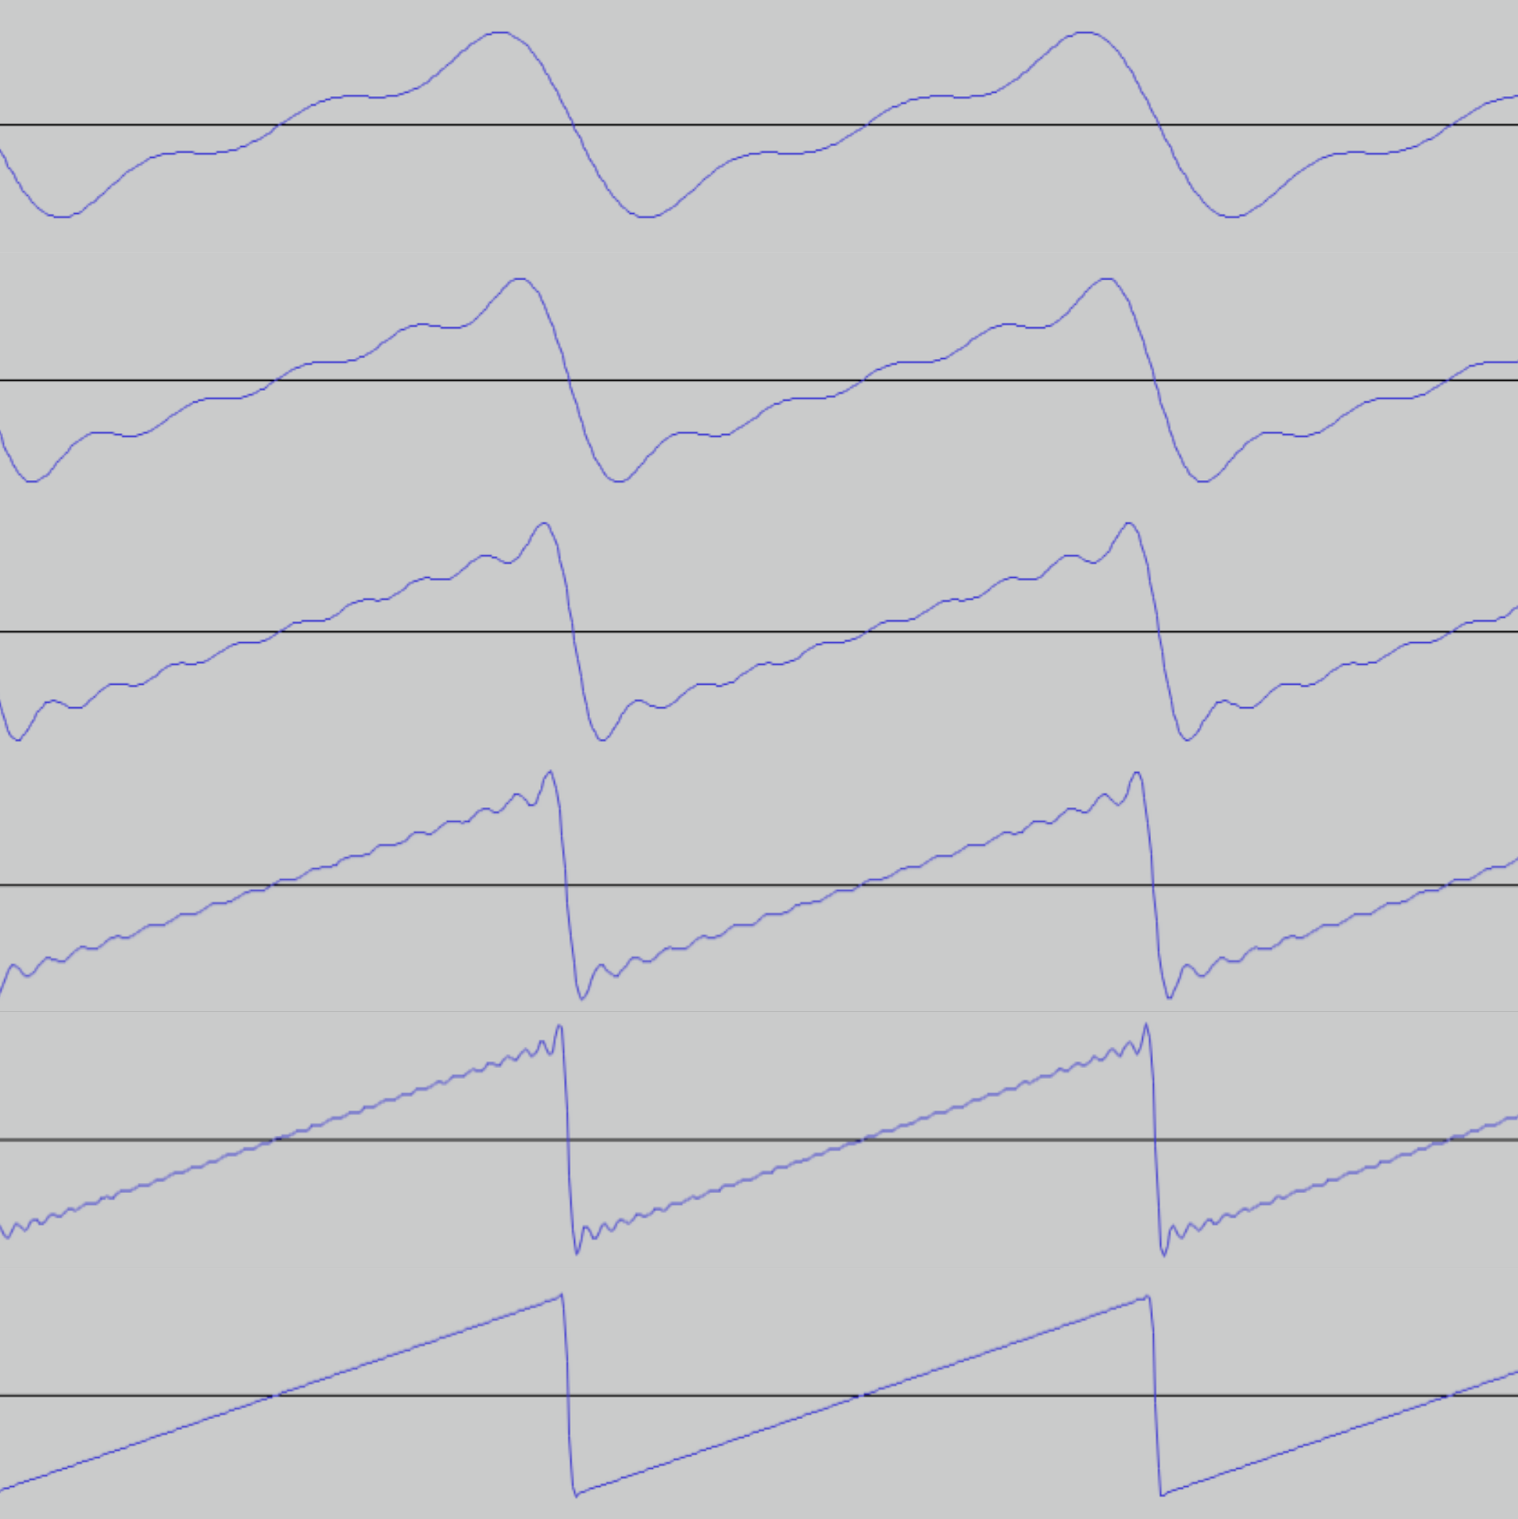
\includegraphics[scale=0.12]{img/ramp}}

    \ttabbox{\caption{C++ code for a ramp wave with 64 partials.} \label{code:aramp}}{\code{aramp.cpp}}

  \end{floatrow}

\end{figure}

\subsubsection{Triangle Waves}

The process of generating triangle waves additively differs from previous waveforms. The amplitude of each partial is no longer the reciprocal of the partial number, $\frac{1}{n}$, but now the inverse of the partial number squared: $\frac{1}{n^2}$. Moreover, the sign of the amplitude alternates for each partial in the series. As for square waves, only odd-numbered partials are used. Mathematically, such a triangle wave is defined as shown in Equation \ref{eq:atri1} or, more concisely, in Equation \ref{eq:atri2}. Figure \ref{fig:tri} displays such a triangle wave with various partial numbers (2,4,8,16,32 and 64) and Table \ref{code:atri} implements C++ code to compute a triangle wave.

\begin{equation}
  f(t) = \sum\limits_{n=1}^\frac{N}{2} \frac{1}{(4n-3)^2}\sin(\omega (4n-3) t) - \frac{1}{(4n-1)^2}\sin(\omega (4n-1) t)
  \label{eq:atri1}
\end{equation}

\begin{equation}
  f(t) = \sum\limits_{n=0}^N \frac{(-1)^n}{(2n+1)^2} \sin(\omega (2n + 1) t)
  \label{eq:atri2}
\end{equation}

\begin{figure}

  \TopFloatBoxes

  \begin{floatrow}

    \ffigbox{\caption{Triangle waves with 2, 4, 8, 16,\\ 32 and 64 partials. Note that already 2 partials\\ produce a very good approximation of a\\ triangle wave.} \label{fig:tri}}{ 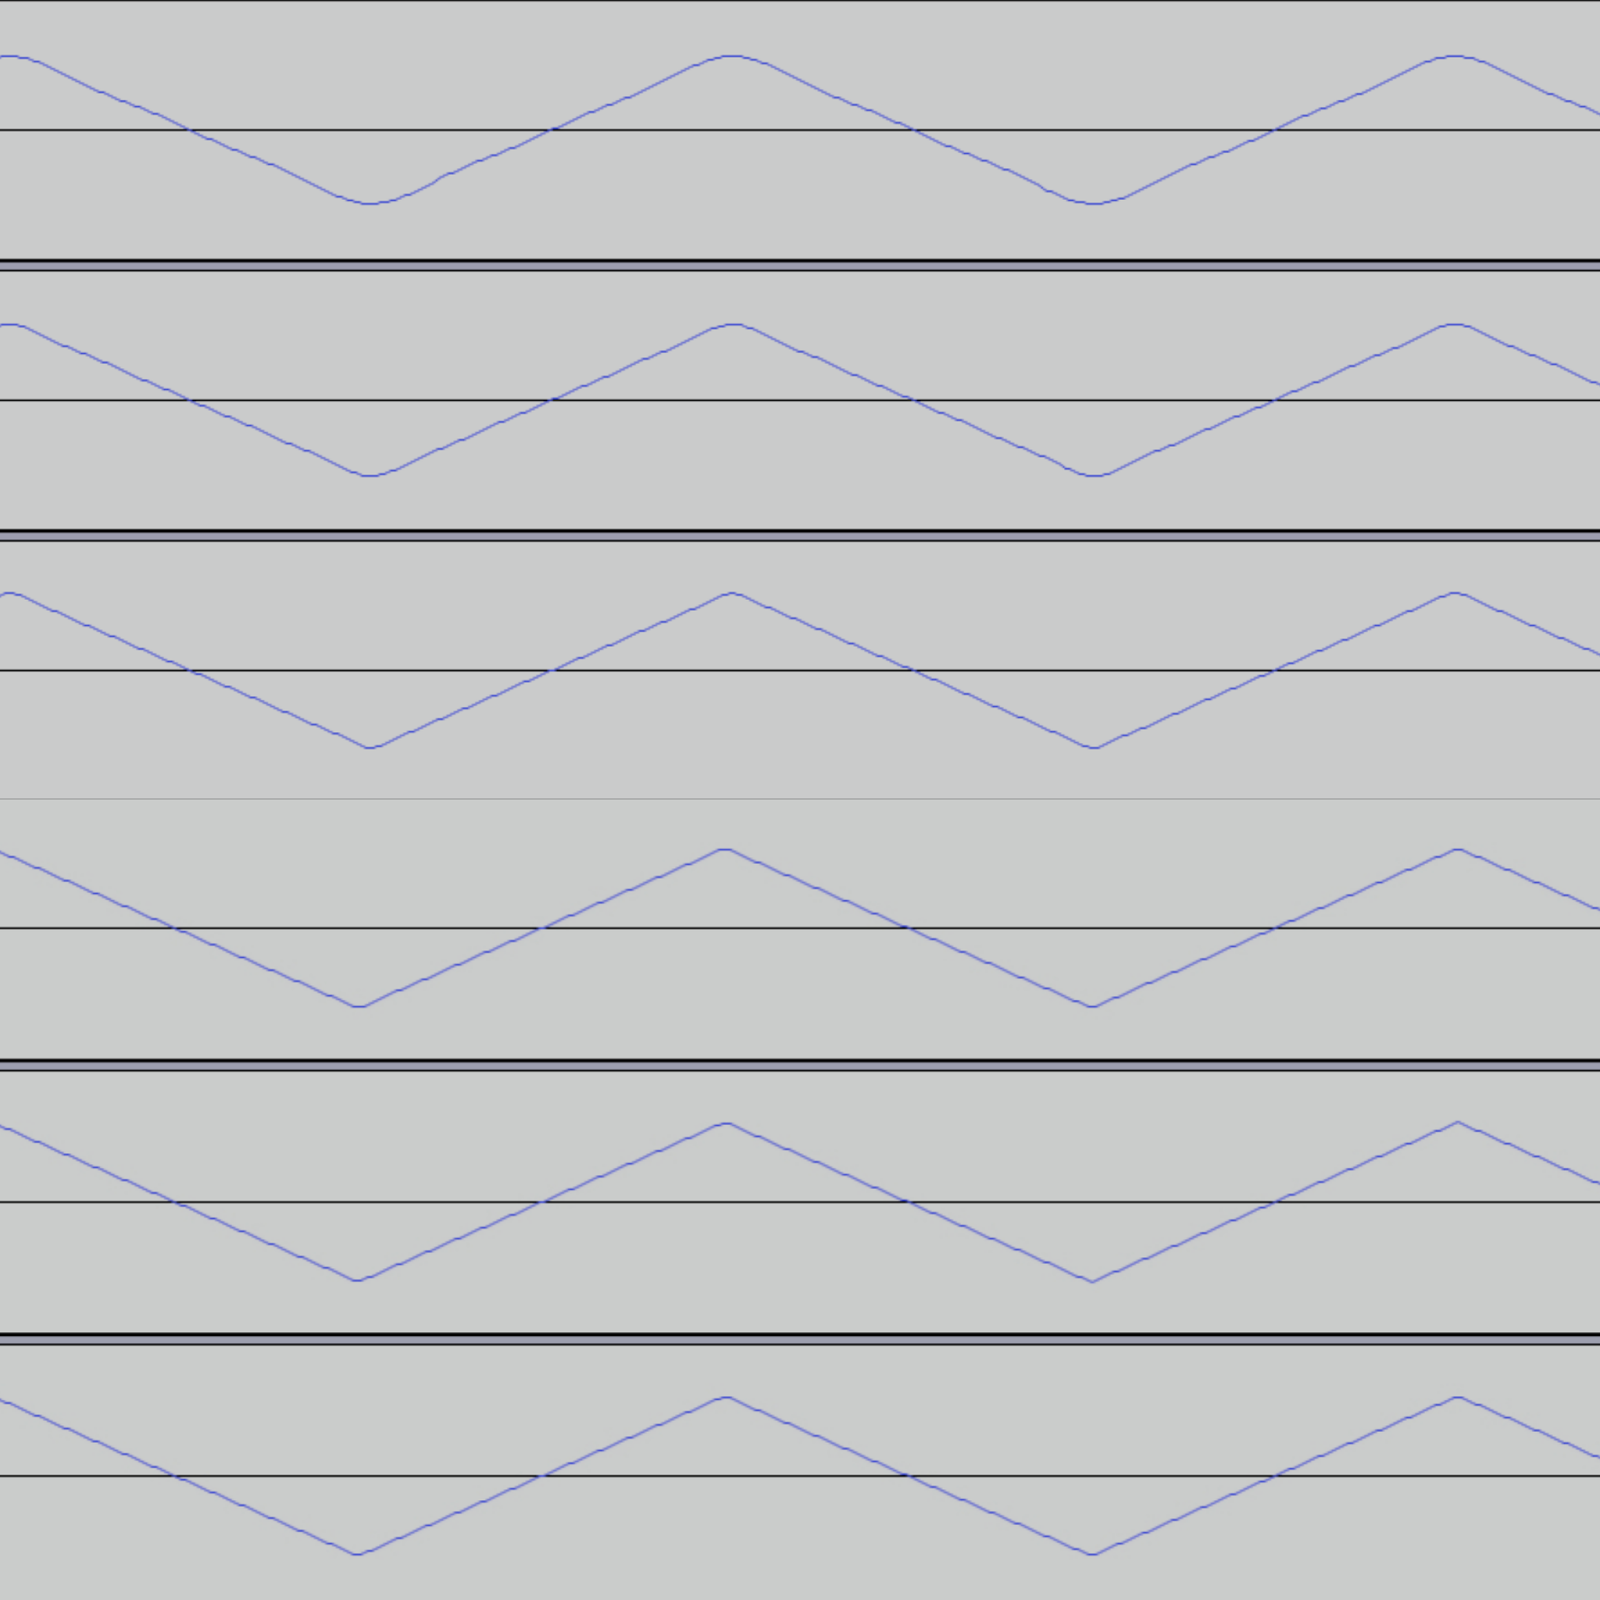
\includegraphics[scale=0.12]{img/tri}}

    \killfloatstyle

    \ttabbox{\code{atri.cpp}}{\caption{C++ code for a triangle wave\\ with 64 partials.} \label{code:atri}}

  \end{floatrow}

\end{figure}

\subsection{Smooth Waveforms}

One noticeable problem with square, sawtooth and ramp waves is that they have very sharp transitions at certain points in their waveforms, such as the square wave at the midpoint, $\frac{T}{2}$, where the amplitude jumps from its maximum to its minimum. While these transitions and jumps in amplitude contribute to the characteristic sound of these waves when used for music, they can pose a problem when they are used for modulation, as sharp transitions in amplitude translate to clicking sounds acoustically. One possible solution to reduce the impact of such transitions would be to overlay an audio envelope directly on the waveform, to bend or smooth the amplitude at the transition points. However, a more effective and direct solution would be to mathematically calculate a waveform that is already smoothed out at these critical points. The following two paragraphs propose a set of empirically determined functions to calculate "smooth" square and sawtooth waves.

\subsubsection{Smooth Square Waves}

Smooth square waves can be calculated mathematically as a set of four power functions with a very large exponent that change their sign after the midpoint. The exponent chosen, 50, was determined entirely experimentally. Equations \ref{eq:ssquareA} to \ref{eq:ssquareD} display the four power functions and their respective range of definition. Figure \ref{fig:ssquare} shows the resulting visualization, where each individual power function is highlighted in a different colour as a visual aid.

\begin{equation}
  a(t) =
  \begin{cases}
    (t - 1)^{50} - 1,& \text{if } 0 \leq t < \frac{T}{4}
  \end{cases}
  \label{eq:ssquareA}
\end{equation}

\begin{equation}
  b(t) =
  \begin{cases}
    (t + 0.5)^{50} - 1,& \text{if } \frac{T}{4} \leq t < \frac{T}{2}
  \end{cases}
  \label{eq:ssquareB}
\end{equation}

\begin{equation}
  c(t) =
  \begin{cases}
    -(t - 1.5)^{50} + 1,& \text{if } \frac{T}{2} \leq t < \frac{3T}{4}
  \end{cases}
  \label{eq:ssquareC}
\end{equation}

\begin{equation}
  d(t) =
  \begin{cases}
    -t^{50} + 1,& \text{if } \frac{3T}{4} \leq t < T
  \end{cases}
  \label{eq:ssquareD}
\end{equation}

\begin{figure}[t!]
  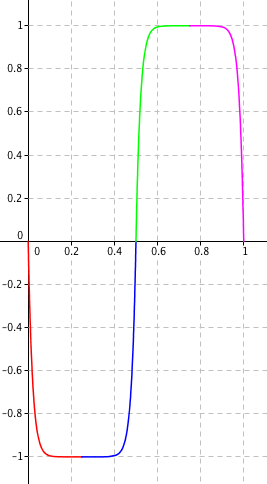
\includegraphics[scale=0.5]{img/ssquare}
  \caption{One period of a smooth square wave as the sum of four piecewise power functions.}
  \label{fig:ssquare}
\end{figure}

\subsubsection{Smooth Sawtooth Waves}

For sawtooth waves, the only critical area of transition is the point at which one period ends and the next begins, as the amplitude jumps back to the maximum from its minimum value. To make this transition smoother, one can use two very steep quadratic functions, one positive and one negative, that intersect at the midpoint of the transition. If one allocates nine tenths of one period for the normal descent of the sawtooth function from its maximum to its minimum, the transition can take place in the last tenth of the period. Equation \ref{eq:ssawA} shows an altered version of the sawtooth wave function introduced in Section 2.2.1 and Equations \ref{eq:ssawB} and \ref{eq:ssawC} the two aforementioned quadratic functions. Figure \ref{fig:ssaw} visualizes the resulting waveform.

\begin{equation}
  a(t) =
  \begin{cases}
    \frac{-2t}{0.9T} + 1 = \frac{-20t}{9T} + 1,& \text{if } 0 \leq t < \frac{9T}{10}
  \end{cases}
  \label{eq:ssawA}
\end{equation}

\begin{equation}
  b(t) =
  \begin{cases}
    400(t-0.9)^2 - 1,& \text{if } \frac{9T}{10} \leq t < \frac{95T}{100}
  \end{cases}
  \label{eq:ssawB}
\end{equation}

\begin{equation}
  c(t) =
  \begin{cases}
    -400(t-1)^2 + 1,& \text{if } \frac{95T}{100} \leq t < T
  \end{cases}
  \label{eq:ssawC}
\end{equation}

\subsubsection{Smooth Ramp Waves}

Smooth ramp waves are created identically to smooth sawtooth waves, except that the sign of all piecewise functions as well as as their offsets change, as shown by Equations \ref{eq:srampA} to \ref{eq:srampC} as well as Figure \ref{fig:sramp}.

\begin{equation}
  a(t) =
  \begin{cases}
    \frac{2t}{0.9T} - 1 = \frac{-20t}{9T} + 1,& \text{if } 0 \leq t < \frac{9T}{10}
  \end{cases}
  \label{eq:srampA}
\end{equation}

\begin{equation}
  b(t) =
  \begin{cases}
    -400(t-0.9)^2 + 1,& \text{if } \frac{9T}{10} \leq t < \frac{95T}{100}
  \end{cases}
  \label{eq:srampB}
\end{equation}

\begin{equation}
  c(t) =
  \begin{cases}
    400(t-1)^2 - 1,& \text{if } \frac{95T}{100} \leq t < T
  \end{cases}
  \label{eq:srampC}
\end{equation}

\begin{figure}

  \TopFloatBoxes

  \begin{floatrow}

    \ffigbox{\caption{A smooth sawtooth wave.} \label{fig:ssaw}}{ 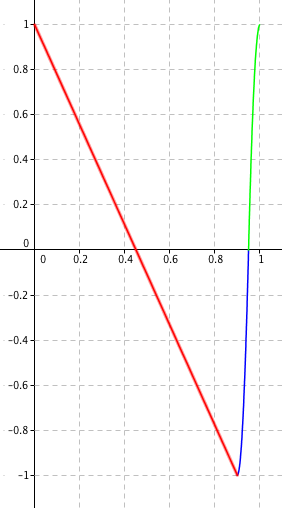
\includegraphics[scale=0.5]{img/ssaw}}

    \ffigbox{\caption{A smooth ramp wave.} \label{fig:sramp}}{ 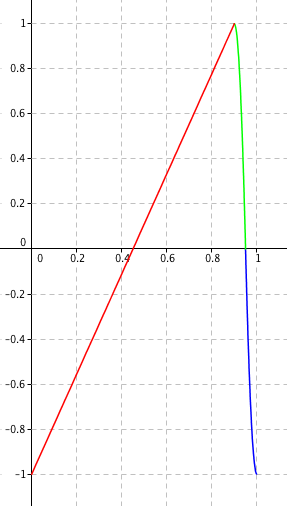
\includegraphics[scale=0.5]{img/sramp}}

  \end{floatrow}

\end{figure}

%\pagebreak

\subsection{Sine Waves with Different Bit Widths}

The bit width of a waveform determines its resolution, i.e. the number of numerical values the amplitude of a signal can take. Common values for the resolution of a waveform are 64 bits, as provided by the C++ double-precision floating-point data type \texttt{double}, or 16 bits, as used by the Waveform Audio File Format (WAVE). Reducing the bit width of a waveform can give the impression of an "old-school" sound, as older synthesis systems from the 20th century were often limited to low bit-widths due to their less advanced hardware, compared to contemporary hardware configurations. Consequently, some digital synthesizers, such as Ableton's Operator, additionally provide waveforms with other bit widths such as 4 or 8 bits. Table \ref{tb:bitw} shows bit width values alongside the number of possibilities a sample can take when the given bit width is used. Note that in general, $n$ bits yield $2^n$ possible values. Figures \ref{fig:sine3} and \ref{fig:sine4} show sine waves with a bit width of 3 and 4 bits, respectively.

\begin{table}[th!]

  \centering

  \begin{tabular}[]{| l | l |}
    \hline
    \rowcolor[gray]{0.8}
    Bit width & Possibilities\\\hline
    2 & 4\\\hline
    3 & 8\\\hline
    4 & 16\\\hline
    8 & 256\\\hline
    16 & 65536\\\hline
    32 & 4294967296\\\hline
    64 & 18446744073709551616\\
    \hline
  \end{tabular}

  \caption{Bit widths alongside the number of possible values a sample can take when the given bit width is used.}

  \label{tb:bitw}

\end{table}

\begin{figure}[th!]
  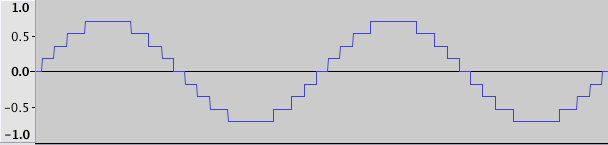
\includegraphics[scale=0.5]{img/sine3}
  \caption{A 3-bit sine wave.}
  \label{fig:sine3}
\end{figure}

\begin{figure}[th!]
  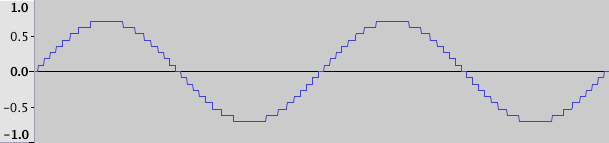
\includegraphics[scale=0.5]{img/sine4}
  \caption{A 4-bit sine wave.}
  \label{fig:sine4}
\end{figure}

\pagebreak

\section{The Gibbs Phenomenon and the Lanczos Sigma Factor}

Examining Figure \ref{fig:gibbsb}, which displays an additively synthesized square wave function with 64 partials, one may observe that additive synthesis, the summation of sine waves to produce complex waveforms, produces an overshoot --- slight ripples or "horns" --- at the ends of each peak and trough of a waveform. This is known as the Gibbs Phenomenon, named after the American scientist Josiah Willard Gibbs who first described it in 1898, and is "the result of summing a finite series of partials rather than the infinite series of partials specified by the Fourier transform" \citebs{67}. Acoustically, this ringing artifact has little influence on the sound of the produced waveform. However, for modulation, this imperfection may render the resulting sound unsatisfactory. A common way to reduce the Gibbs Phenomenon is to apply the Lanczos Sigma ($\sigma$) Factor to each partial of a Fourier Series. This is often called \emph{sigma-approximation}. The definition of the Lanczos Sigma Factor is given in Equation \ref{eq:lanczos}, where $n$ is the current partial number and $M$ the total number of partials in a Fourier Summation. In the \texttt{additive} function shown in Tables \ref{code:add1} and \ref{code:add2}, the Lanczos Sigma Factor is implemented in lines 48 to 54. Figure \ref{fig:gibbsa} shows the same square wave from Figure \ref{fig:gibbsb} after sigma-approximation.

\begin{equation}
  \sigma = sinc(\frac{n\pi}{M}) = \frac{\sin(\frac{n\pi}{M})}{\frac{n\pi}{M}}
  \label{eq:lanczos}
\end{equation}

\begin{figure}
  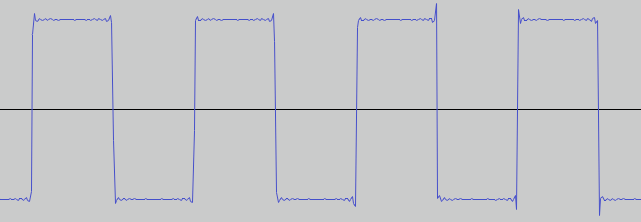
\includegraphics[scale=0.5]{img/gibbsb}
  \caption{An additively synthesized square wave with 64 partials before sigma-approximation.}
  \label{fig:gibbsb}
\end{figure}

\begin{figure}
  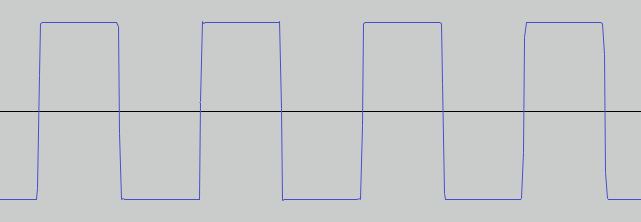
\includegraphics[scale=0.5]{img/gibbsa}
  \caption{An additively synthesized square wave with 64 partials after sigma-approximation.}
  \label{fig:gibbsa}
\end{figure}

\pagebreak

\section{Wavetables}

Following the discussion of the creation of complex waveform, the two options for playing back waveforms in a digital synthesis system must be examined: continuous real-time calculation of waveform samples or lookup from a table that has been calculated once and then written to disk --- a so-called Wavetable. To keep matters short, the second method was found to be computationally more efficient and thus the better choice, as memory is a more easily expended resource than computational speed.

\subsection{Implementation}

A Wavetable is a table (practically speaking an array) in which one stores pre-calculated waveform amplitude values for lookup. This way, the computation of individual samples as shown in Sections 2.2.1 and 2.2.2 can be replaced by the incrementing of a table index variable and retrieval of samples by dereferencing of the array at the current index. If a table holds sample values for one period of a waveform, at a frequency of $1 Hz$, the frequency of the waveform can be adjusted during playback by multiplying the increment value by some factor other than one. "For example, if we increment by two [instead of one], we scan the table in half the time and produce a frequency twice the original frequency. Other increment values will yield proportionate frequencies." \citebs{80-81} The fundamental increment for a table index, $i_{fund}$, the value by which a table index must be incremented after each sample to traverse a waveform at a frequency of $1 Hz$, given the table length $L$ and the samplerate $f_{s}$, is shown in Equation \ref{eq:fundincr}. To alter the frequency $f$ of the played-back waveform, Equation \ref{eq:otherincr} should be used to calculate the appropriate increment value $i$.

\begin{equation}
  i_{fund} = \frac{L}{f_{s}}
  \label{eq:fundincr}
\end{equation}

\begin{equation}
  i = i_{fund} \cdot f = \frac{L}{f_{s}} \cdot f
  \label{eq:otherincr}
\end{equation}

\subsection{Interpolation}

For almost all configurations of frequencies, table lengths and sample rates, the table index $i$ produced by Equation \ref{eq:otherincr} will not be an integer. Since using a floating point number as an index for an array is a syntactically illegal operation in C++, there are two options. The first is to truncate or round the table index to an integer, thus "introducing a quantization error into the signal [...]". This is obviously a suboptimal solution which would result in a change of phase and consequently distortion. \citebs{84} The second option, interpolation, tries to approximate the true value from the sample at the current index and at the subsequent one. Interpolation is achieved by summation of the sample value at the floored, integral part of the table index, $\left \lfloor{i}\right \rfloor$, with the difference between this sample and the sample value at the next table index, $\left \lfloor {i}\right \rfloor + i$, multiplied by the fractional part of the table index, $i - \left \lfloor {i}\right \rfloor$. Table \ref{code:pseudointerp} displays the calculation of a sample by means of interpolation in pseudo-code and Table \ref{code:interp} in C++. (based on pseudo-code, Mitchell, 2008, p. 85)

\begin{table}
  \code{interpolation.pseudo}
  \caption{An interplation algorithm in pseudo-code.}
  \label{code:pseudointerp}
\end{table}

\begin{table}
  \code{interpolation.cpp}
  \caption{Full C++ template function to interpolate a value from a table, given a fractional index. }
  \label{code:interp}
\end{table}

\subsection{Table Length}

The length of the Wavetable must be chosen carefully to be both memory efficient and at the same time provide a decently accurate waveform resolution. An equation to calculate the size of a single wavetable in Kilobytes is given by Equation \ref{eq:tablesize}, where L is the table length and $N$ the number of bytes provided by the resolution of the data type used for samples, e.g. 8 bytes for the double-precision floating-point data type \texttt{double}.

\begin{equation}
  Size = \frac{L \cdot N}{1024}
  \label{eq:tablesize}
\end{equation}

\noindent Daniel R. Mitchell advises that the length of the table be a power of two for maximum efficiency. \citebs{86} Moreover, during an E-Mail exchange with Jari Kleimola, author of the 2005 master's thesis titled "Design and Implementation of a Software Sound Synthesizer", it was discovered that "as a rule of thumb", the table length should not exceed the processor cache size. A relevant excerpt of this e-mail exchange is depicted in Figure \ref{fig:jari}.

\begin{figure}
  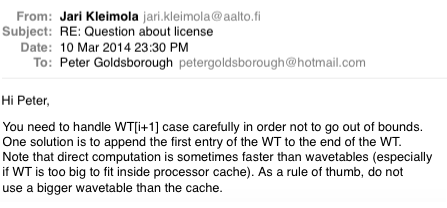
\includegraphics[scale=0.7]{img/jari}
  \caption{An excerpt of an E-Mail exchange with Jari Kleimola.}
  \label{fig:jari}
\end{figure}

\noindent Considering both pieces of advice, it was decided that a Wavetable size of 4096 ($2^12$), which translates to 32 KB of memory, would be suitable.\\

\noindent One important fact to mention, also discussed by Jari Kleimola as seen in Figure \ref{fig:jari}, is that because the interpolation algorithm from Table \ref{code:interp} must have access to the sample value at index $i+1$, $i$ being the current index, an additional sample must be appended to the Wavetable to avoid a \texttt{BAD\_ACCESS} error. This added sample usually has the same value as the first sample in the table to avoid a discontinuity. Therefore, the period of the waveform actually only fills 4095 of the 4096 indices of the Wavetable, as the 4096th sample is equal to the first.

\subsection{File Format}

For maximum efficiency, the Wavetables are not created at program startup but read from a binary file. To prevent the synthesizer program from accidentally reading faulty files, some simple identification string must be added to the file. Therefore, Wavetable files contain a 6-char ID string with the name of the synthesizer, Anthem, after which the 32 KB of Wavetable data follow. Additionally, Wavetable files end with a \texttt{.wavetable} file extension. Table \ref{code:wtfile} displays a function to read such a Wavetable file and Figure \ref{fig:wtfile} shows the first few bytes of a Wavetable file when opened as plain-text. The total size of a Wavetable file is exactly 32774 bytes, 32768 bytes (32KB) of Wavetable data and 6 bytes for the ID string.

\begin{table}[t!]
  \code{file.cpp}
  \caption{C++ code to read a Wavetable file. }
  \label{code:wtfile}
\end{table}

\begin{figure}[h!]
  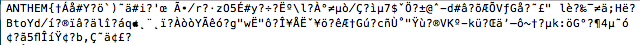
\includegraphics[scale=0.7]{img/wtfile}
  \caption{The first few bytes of a Wavetable file.}
  \label{fig:wtfile}
\end{figure}

\section{Noise}

A noisy signal is a signal in which some or all samples take on random values. Generally, noise is considered as something to avoid, as it may lead to unwanted distortion of a signal. Nevertheless, noise can be used as an interesting effect when creating music. Its uses include, for example, the modeling of the sound of wind or the crashing of water waves against the shore of a beach. Some people enjoy the change in texture noise induces in a sound, others find noise relaxing and even listen to it while studying. \citebs{76} Unlike all audio signals\footnotemark{} presented so far, noise cannot\footnotemark{} be stored in a Wavetable, as it must be random throughout its duration and not repeat periodically for a proper sensation of truly \emph{random} noise.

\footnotetext{The term "waveform" would be incorrect here, as noise is not periodic and thus cannot really be seen as a waveform.}

\footnotetext{Noise could theoretically be stored in a Wavetable, of course. However, even a very large Wavetable destroys the randomness property to some extent and would thus invalidate the idea behind noise being truly random.}

\subsection{Colors of Noise}

The \emph{color} of a noise signal describes, acoustically speaking, the \emph{texture} or \emph{timbre} \footnotemark{} of the sound produced, as well as, scientifically speaking, the spectral power density and frequency content of the signal. The following paragraphs will examine and explain the creation of various noise colors, namely white, pink, red, violet and blue noise.

\footnotetext{Timbre is a rather vague term used by musicians and audio engineers to describe the properties, such as pitch, tone and intensity, of an audio signal's sound that distinguish it from other sounds. The \emph{Oxford Dictionary of English} defines timbre as "the character or quality of a musical sound or voice as distinct from its pitch and intensity".}

\subsubsection{White Noise}

White noise is a random signal in its purest and most un-filtered form. In such a signal, all possible frequencies are found with a uniform probability distribution, meaning they are distributed at equal intensity throughout the signal. The association of noise with colors actually stems from the connection between white noise and white light, which is said to be composed of almost all color components at an approximately equal distribution. Figure \ref{fig:wnoise} shows a typical white noise signal in the time domain, Figure \ref{fig:wnoisez} gives a close-up view of Figure \ref{fig:wnoise}, Figure \ref{fig:wnoisef} displays the frequency spectrum of a white noise signal and Table \ref{code:wnoise} shows the implementation of a simple C++ class to produce white noise.

\begin{figure}[h!]
  \sidecap{A typical white noise signal.}{fig:wnoise}
  {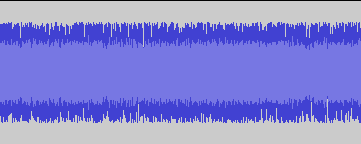
\includegraphics[scale=0.62]{img/wnoise}}
\end{figure}

\begin{figure}[h!]
  \sidecap{A close-up view of Figure \ref{fig:wnoise}. This Figure shows nicely how individual sample values are completely random and independent from each other. }{fig:wnoisez}
  {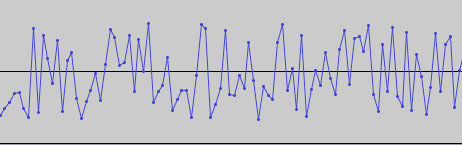
\includegraphics[scale=0.5]{img/wnoisez}}
\end{figure}

\begin{figure}[h!]
  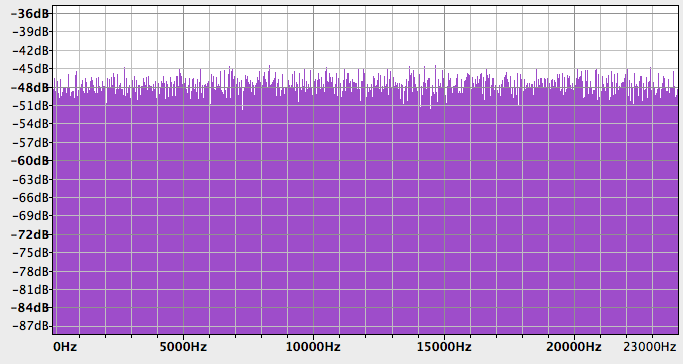
\includegraphics[scale=0.6]{img/wnoisef}
  \caption{The signal from Figures \ref{fig:wnoise} and \ref{fig:wnoisez} in the frequency domain. This frequency spectrum analysis proves the fact that white noise has a "flat" frequency spectrum, meaning that all frequencies are  distributed uniformly and at (approximately) equal intensity. }
  \label{fig:wnoisef}
\end{figure}

\begin{table}
  \code{wnoise.cpp}
  \caption{A simple C++ class to produce white noise. \texttt{rgen\_} is a random number generator following the Mersenne-Twister algorithm, to retrieve uniformly distributed values from the \texttt{dist\_} distribution in the range of -1 to 1. \texttt{tick()} returns a random white noise sample. }
  \label{code:wnoise}
\end{table}

\subsubsection{Pink Noise}

Pink noise, sometimes referred to as $\frac{1}{f}$ noise, is white noise filtered with a 3dB/octave low-pass filter. In contrast to white noise, which has equal energy \emph{per frequency component}, pink noise has equal energy \emph{per octave}. This is a significant difference as humans hear on the basis of octaves (logarithmically), and not completely linearly, meaning that for the human ear the difference between 400 and 800 Hertz (one octave) sounds the same as the octave jump between 6 KHz and 11 Khz, even though the absolute difference between thoes two ranges is 4.6 Khz! To address this phenomenon, pink noise has more energy in the lower, narrower octave ranges and less energy in the wider, higher octave ranges. Therefore, the few high intensity values in the low frequency bands add up to equal the sum of lower intensity values in the wider, higher frequency octave bands. Figure \ref{fig:pnoisef} displays the frequency spectrum of pink noise. In the time domain, pink noise looks more or less like white noise, as can be seen in Figure \ref{fig:pnoiset}.

\begin{figure}[t!]
  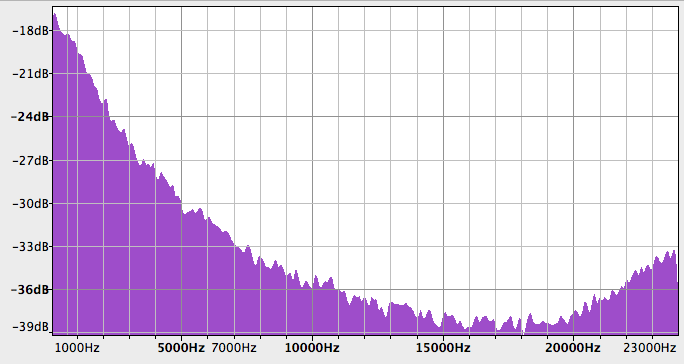
\includegraphics[scale=0.6]{img/pnoisef}
  \caption{The frequency spectrum of pink noise. Note that the filter with which white noise was transformed into pink noise, discussed in a later chapter, is not perfect, resulting in the increase in frequency intensity towards the end of the spectrum. Ideally, the intensity should decrease linearly.}
  \label{fig:pnoisef}
\end{figure}

\begin{figure}[t!]
  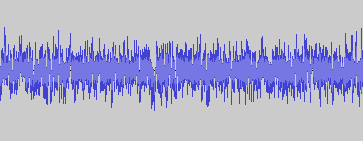
\includegraphics[scale=0.7]{img/pnoiset}
  \caption{Pink noise in the time domain.}
  \label{fig:pnoiset}
\end{figure}

\subsubsection{Red Noise}

Red Noise has an energy decrease of 6dB/Octave. Another method of generating red noise besides filtering white noise appropriately is integrating a white noise signal, as shown in Equation \ref{eq:rnoise}. Red noise is also called "Brown" or "Brownian" noise. This name is not given for its visual equivalent, but rather for it's resemblance to a signal produced by Brownian motion or "Random Walk", "the erratic random movement of microscopic particles in a fluid, as a result of continuous bombardment from molecules of the surrounding medium." (Oxford Dictionary of English, 2003). Figure \ref{fig:rnoisef} shows a red noise signal in the frequency domain and Figure \ref{fig:rnoiset} in the time domain.

\begin{equation}
  N_{red}(t) = \int_{0}^{t} N_{white}(t)dt
  \label{eq:rnoise}
\end{equation}

\begin{figure}[t!]
  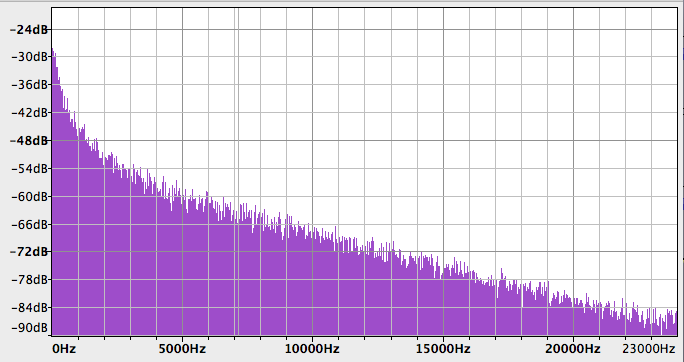
\includegraphics[scale=0.6]{img/rnoisef}
  \caption{Red noise in the frequency domain.}
  \label{fig:rnoisef}
\end{figure}

\begin{figure}[t!]
  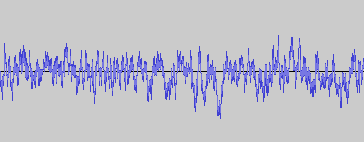
\includegraphics[scale=0.7]{img/rnoiset}
  \caption{Red noise in the time domain.}
  \label{fig:rnoiset}
\end{figure}

\subsubsection{Blue Noise}

Wherease pink and red noise show a decrease in intensity per frequency component, blue noise exhibits an \textbf{increase} in intensity by 3dB/Octave, making it sound like a high-pitched version of white noise. Blue noise can be created by making the filter used for pink noise a high-pass filter instead of a low-pass one, meaning that higher frequencies are filtered less than lower ones. Figure \ref{fig:bnoisef} shows a frequency spectrum of the blue noise created for the purpose of this thesis. The reader may question as to why the spectrum shown looks nothing like what was just described as the ideal spectrum of blue noise. As matter of fact, it was discovered that a frequency spectrum of this kind, combined with a decreased gain of -3dB, produces the same sound as an ideal blue noise signal. In the time domain, blue noise looks similar to the white noise depicted in Figure \ref{fig:wnoise}.

\begin{figure}[hb!]
  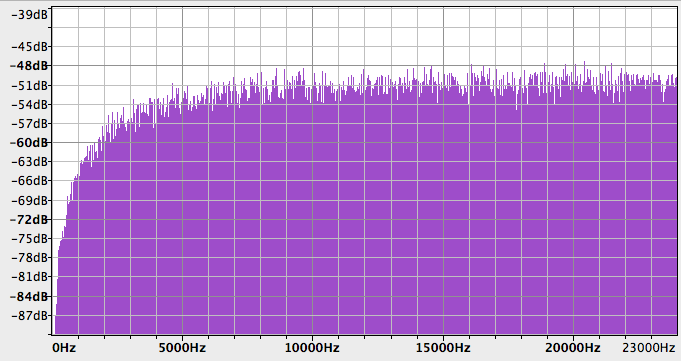
\includegraphics[scale=0.6]{img/bnoisef}
  \caption{Blue noise in the frequency domain.}
  \label{fig:bnoisef}
\end{figure}

\pagebreak

\subsubsection{Violet Noise}

What blue noise is to pink noise, violet noise is to red noise. Violet noise increases by 6dB per octave and can also be created by differentiating a white noise signal, just as red noise is the result of integrating white noise. Acoustically, violet noise sounds like a very high-pitched "hissing" sound. Equation \ref{eq:vnoise} shows how violet noise can be produced as a derivative of white noise and Figure \ref{fig:vnoisef} shows the frequency response of a violet noise signal.

\begin{equation}
  N_{violet} = \frac{dN_{white}(t)}{dt}
  \label{eq:vnoise}
\end{equation}

\begin{figure}
  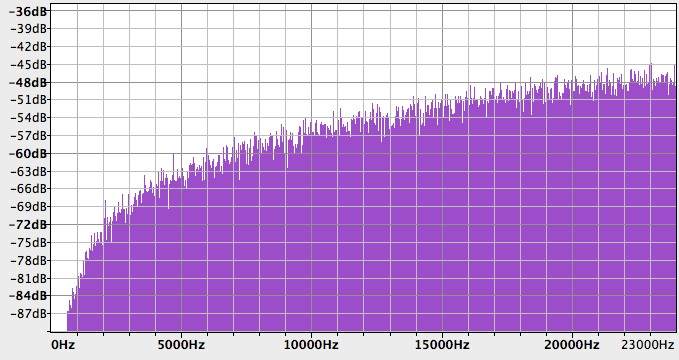
\includegraphics[scale=0.6]{img/vnoisef}
  \caption{The frequency spectrum of a violet noise signal.}
  \label{fig:vnoisef}
\end{figure}

\chapter{Modulating Sound}

One of the most interesting aspects of any synthesizer, digital as well as analog, is its capability to modify or \emph{modulate} sound in a variety of ways. To modulate a sound means to change its amplitude, pitch, timbre, or any other property of a signal to produce an, often entirely, new sound. This chapter will examine and explain two of the most popular means of modulation in a digital synthesis system, Envelopes and Low Frequency Oscillators (LFOs).

\section{Envelopes}

When a pianist hits a key on his piano, the amplitude of the sound produced increases from zero, no sound, to some maximum amplitude which depends on a multitude of factors such as how hard the musician pressed the key, what material the piano string is made of, the influence of air friction and so on. After reaching the maximum loudness, the amplitude decreases until the piano string stops oscillating, resulting in renewed silence. To model such an evolution of amplitude over time, digital musicians use a modulation technique commonly referred to as an "Envelope".

\subsection{Envelope segments}

The following sections outline the creation of and terminology used for single segments of an envelope.

\subsubsection{ADSR}

A common concept associated with Envelopes is "ADSR", which stands for "Attack, Decay, Sustain, Release". These four terms name the four possible states an Envelope segment can take on. An Attack segment is any segment where the initial amplitude, at the start of a segment, is less than the final amplitude, at the end of the segment --- the amplitude increases. Conversely, a Decay segment signifies a decrease in amplitude from a higher to a lower value. When the loudness of a signal stays constant for the full duration of an interval, this interval is termed a "Sustain" segment. While the three segment types just mentioned all describe the modulation of a signal's loudness when the key of a piano or synthesizer is still being pressed, the last segment type, a "Release" segment, refers to the change in loudness once the key is \emph{released}. Figure \ref{fig:adsr} depicts an abstract representation of a typical ADSR envelope. Figure \ref{fig:envb} shows a 440 Hz sine wave before the application of an ADSR envelope and Figure \ref{fig:enva} displays the same signal after an ADSR envelope has been applied to it.

\begin{figure}[p!]
  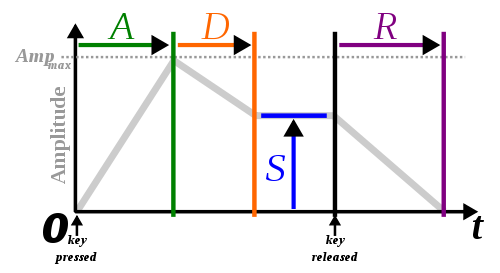
\includegraphics[scale=0.8]{img/adsr}
  \caption{An Envelope with an Attack, a Decay, a Sustain and finally a Release segment. Source: \protect\url{http://upload.wikimedia.org/wikipedia/commons/thumb/e/ea/ADSR_parameter.svg/500px-ADSR_parameter.svg.png}}
  \label{fig:adsr}
\end{figure}

\begin{figure}[p!]
  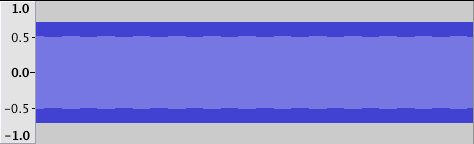
\includegraphics[scale=0.8]{img/envb}
  \caption{A 440 Hz sine wave.}
  \label{fig:envb}
\end{figure}

\begin{figure}[p!]
  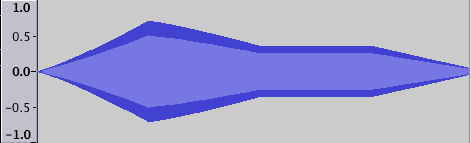
\includegraphics[scale=0.8]{img/enva}
  \caption{The same signal from Figure \ref{fig:envb} with an ADSR Envelope overlayed on it.}
  \label{fig:enva}
\end{figure}

\subsubsection{Mathematical Definition and Rate Types}

Mathematically, an Envelope segment can be modeled using a simple power function of the general form presented in Equation \ref{eq:power}, where $a_{final}$ is the final amplitude at the end of the segment, $a_{start}$ the initial amplitude at the beginning of the segment and $r$ the parameter responsible for the shape or "rate" of the segment. When $r$, which must kept between $0$ and $\infty$ (practically speaking some value around $10$), is equal to $1$, the segment has a linear rate and is thus a straight line connecting the initial amplitude with the final loudness. If $r$ is greater than 1, the function becomes a power function and consequently exhibits a non-linear increase or decrease in amplitude. Lastly, if $r$ is less than 1 but greater than 0, the function is termed a "radical function", since any term of the form $x^\frac{a}{b}$ can be re-written to the form $\sqrt[b]{x^a}$, where the numerator $a$ becomes the power of the variable and the denominator $b$ the radicand. Figure \ref{fig:rates} displays an envelope whose first segment has $r = 2$, a quadratic increase, after which the sound decays linearly, before increasing again, this time $r$ being equal to $\frac{1}{2}$ (a square root function). A C++ class for single Envelope segments is shown in Listing \ref{code:envseg}.

\begin{equation}
  a(t) = (a_{final} - a_{start}) \cdot t^r + a_{start}
  \label{eq:power}
\end{equation}

\begin{figure}
  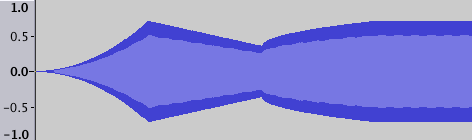
\includegraphics[scale=0.7]{img/rates}
  \caption{An envelope where $r$ is equal to 2, then to 1, then to 0.5.}
  \label{fig:rates}
\end{figure}

\subsection{Full Envelopes}

Creating full Envelopes with a variable number of segments requires little more work than implementing a state-machine, which checks whether the current sample count is greater than the length of the Envelope segment currently active. If the sample count is still less than the length of the segment, one retrieves Envelope values from the current segment, else the Envelope progresses to the next segment. Additionally, it should be possible for the user to loop between segments of an Envelope a variable number of times before moving on to the release segment. Table \ref{code:envsegseq} displays two member functions of an Envelope class created for this thesis, which return an Envelope value from the current Envelope segment and allow for the update of the sample count.\\

\begin{table}
  \code{envsegseq.cpp}
  \caption{Two member functions of the EnvSegSeq class (Envelope Segment Sequence).}
  \label{code:envsegseq}
\end{table}

\noindent Envelopes have many uses. Some require flexible segments which allow for the adjusting of individual segments' lengths, others need all segments to have a constant length. Some give the user the possibility to modulate individual segments by making them behave like a sine function, others do not. Fortunately, C++'s inheritance features make it very easy and efficient to construct such a variety of different classes that may or may not share relevant features. The inheritance diagram for the final \texttt{Envelope} class created for the purpose of this thesis reflects how all of these individual class can play together to yield the wanted features for a class. This inheritance diagram is displayed in Figure \ref{fig:envelope-inherit}.

\begin{figure}
  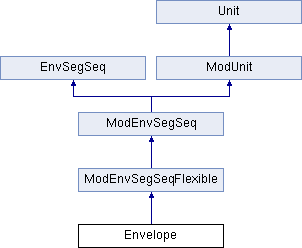
\includegraphics[scale=0.7]{img/envelope-inherit}
  \caption{The inheritance diagram for the \texttt{Envelope} class. The \texttt{Unit} and \texttt{ModUnit} classes are two abstract classes that will be explained in later parts of this thesis.}
  \label{fig:envelope-inherit}
\end{figure}

\section{Low Frequency Oscillators}

A Low Frequency Oscillator, abbreviated "LFO", is an oscillator operating at very low frequencies, typically in the range below human hearing (0-20 Hz), used solely for the purposes of modulating other signals. The most common parameter to be modulated by an LFO in a synthesizer is the amplitude of another oscillator, to produce effects such as the well known "vibrato" effect. In this case, were the frequency of the LFO to be in the audible range, one would use the term Amplitude Modulation (AM), which is also a method for synthesizing sound. Moreover, Amplitude Modulation is one of the two main techniques for transmitting information over electro-magentic waves, alongside Frequency Modulation (FM), but that is a different subject, entirely. Equation \ref{eq:lfoam} shows how an LFO can be used to change the amplitude of another oscillator\footnote{This is the same equation as for AM.}. Figure \ref{fig:lfo1} shows a 440 Hz sine wave, Figure \ref{fig:lfo2} displays the same sine wave now modulated by a 2 Hz LFO and in Figure \ref{fig:lfo3} the frequency of the LFO has been increased to 20 Hz to produce a vibrato effect. It should be noted that an LFO can also modulate any other parameter, such as the rate of an Envelope segment.

\begin{equation}
  O(t) = (A_{osc} + (A_{lfo} \cdot sin(\omega_{lfo}t + \phi_{lfo}))) \cdot sin(\omega_{osc}t + \phi_{osc})
  \label{eq:lfoam}
\end{equation}

\begin{figure}[h!]
  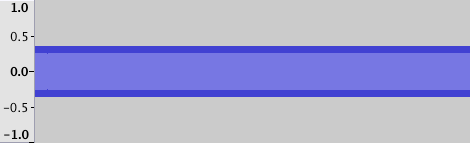
\includegraphics[scale=0.5]{img/lfo1}
  \caption{A 440 Hz sine wave.}
  \label{fig:lfo1}
\end{figure}

\begin{figure}[h!]
  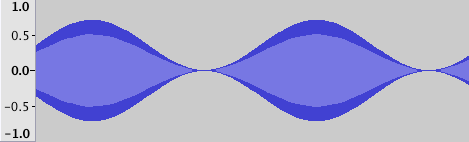
\includegraphics[scale=0.5]{img/lfo2}
  \caption{The sine wave from Figure \ref{fig:lfo1} modulated by an LFO with a frequency of 2 Hertz. Note how the maximum amplitude of the underlying signal now follows the waveform of a sine wave. Because the LFO's amplitude is the same as that of the oscillator (the "carrier" wave), the loudness is twice as high at its maximum, and zero at its minimum.}
  \label{fig:lfo2}
\end{figure}

\begin{figure}[h!]
  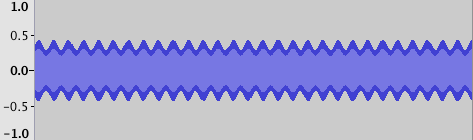
\includegraphics[scale=0.5]{img/lfo3}
  \caption{The sine wave from Figure \ref{fig:lfo1} modulated by an LFO with a frequency of 20 Hertz. This signal is said to have a "vibrato" sound to it.}
  \label{fig:lfo3}
\end{figure}

\pagebreak

\noindent Concerning the implementation of an LFO in a computer program, the process could be as simple as re-naming a class used for an oscillator:

\begin{lstlisting}
  typedef OscillatorClass LFOClass.
\end{lstlisting}

\noindent In the synthesizer created for this thesis, called \emph{Anthem}, the distinction between an LFO and an oscillator is the possibility to modulate an LFO's parameters, for example using an Envelope or another LFO, whereas the \texttt{Oscillator} class is an abstract base class whose sole purpose is to be an interface to a Wavetable. This property of the \texttt{Oscillator} class is used by both the \texttt{LFO} and the \texttt{Operator} class, who both inherit from the \texttt{Oscillator} class. The \texttt{Operator} class is the sound generation unit the user actually interfaces with from the Graphical User Interface (GUI) of Anthem. It is derived from the \texttt{Oscillator} class because it ultimately needs to generate sound samples, but it is its own class because it has various other features used for sound synthesis. These features are discussed in a later chapter. The relationships just described lead to the inheritance diagram shown in Figure \ref{fig:osc-derived}.

\begin{figure}[h!]
  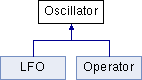
\includegraphics[scale=0.9]{img/osc-derived}
  \caption{Inheritance diagram showing the relationship between an \texttt{LFO}, an \texttt{Operator} and their base class, the \texttt{Oscillator} class.}
  \label{fig:osc-derived}
\end{figure}

\subsection{LFO Sequences}

A common sight in many modern digital synthesizers, such as Native Instruments'\footnotemark{} "Massive" synthesizer, is a form of step-sequencer for Low Frequency Oscillators. This modulation unit is essentially a synthesis between the concept of an Envelope and that of an LFO. It has a variable number of segments of fixed length, each with their own LFO to change the waveform of the segment. Figure \ref{fig:lfoseq} displays what Native Instruments calls a "Stepper".\\

\footnotetext{"Native Instruments is a technology company that develops software and hardware for music production and DJ-ing", based out of Berlin, Germany. Source: \emph{Wikpedia:} \url{http://en.wikipedia.org/wiki/Native_Instruments}. Homepage: \url{http://www.native-instruments.com/en/}}

\begin{figure}
  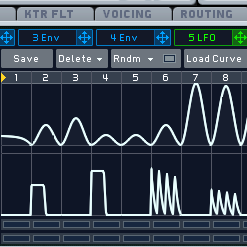
\includegraphics[scale=0.6]{img/lfoseq}
  \caption{An LFO sequence, here named a "Stepper". Source: \protect\url{http://www.askaudiomag.com/articles/massives-performer-and-stepper-lfos}}
  \label{fig:lfoseq}
\end{figure}

\noindent For the purpose of this thesis, such an LFO sequence was created. Regarding the implementation in C++, there is little difference between an LFO Sequence and an Envelope Segment Sequence, except for the fact that now each individual segment has an LFO that can be accessed through the interface of the class to change the parameters or the waveform of each LFO. One of the two parameters that deserves to be discussed, however, is the frequency or "rate" of such an LFO sequence. Just like the frequency of an oscillator describes the number of cycles its waveform completes every second, the rate of an LFO Sequence determines how often the entire sequence is traversed in one second. Practically speaking, this involves adjusting the length of individual segments in such a way that the combined length equals the wanted duration. To give an example: if the user wishes to change the rate of an LFO Sequence with 10 segments to 1 Hz, each individual segment must have a duration of 0.1 seconds (100 milliseconds), so that at the end of the sequence, exactly $10 \text{ segments} \cdot 0.1 \text{ seconds} = 1 \text{ second}$ will have passed. The length of a single segment can be derived from Equation \ref{eq:lfoseq1}, where $r$ is the rate of the LFO Sequence and $N$ the number of segments in the sequence.

\begin{equation}
  l_{seg} = \frac{1}{r \cdot N}
  \label{eq:lfoseq1}
\end{equation}

\noindent The second parameter worthy of mentioning is the frequency of individual segments' modulation LFOs. As mentioned, the frequency of an oscillator or of an LFO sets the cycles per second of their waveform. However, when the length of a single segment in an LFO sequence is only very small, e.g. 100 milliseconds, having an LFO modulate the segment at a common frequency of, say, 1 Hz, would mean that only one tenth of the LFO's period is completed. To have the LFO complete a full cycle, the user would have to adjust the frequency of the LFO in such a way that it can complete one period within the duration of the segment (in this case, 10 Hz). This may still seem like a manageable task for the user. However, once parameter values become a little more complicated, giving birth to cases where the user has to figure out that to have 5 cycles in a segment with a duration of 0.4 seconds, the frequency needs to be exactly 12.5 Hz, the objective reader must admit that this is not intuitive behaviour. Therefore, it was decided that for modulation LFOs in LFO sequences, the rate should not be defined as cycles per second, but as cycles per \emph{segment}. This means that setting the rate of a segment's LFO to 5 Hertz results in 5 cycles per second \emph{regardless} of the segment's duration. Naturally, the task of calculating the correct frequency for the LFO still has to be performed by the computer program. The \emph{real} frequency can be calculated using Equation \ref{eq:lfoseq2} when the duration $d$ is in seconds and Equation \ref{eq:lfoseq3} when the duration is in samples, as is the case for a digital synthesizer. In both Equations $f_{displayed}$ stands for the frequency the user specifies, the cycles per segment, and $f_{real}$ for the actual frequency in cycles per second. Furthermore, in Equation \ref{eq:lfoseq3}, $f_{s}$ denotes the sample rate.

\begin{equation}
  f_{real} = \frac{f_{displayed}}{d}
  \label{eq:lfoseq2}
\end{equation}

\begin{equation}
  f_{real} = \frac{f_{s}}{d} \cdot f_{displayed}
  \label{eq:lfoseq3}
\end{equation}

\begin{table}[t!]
  \code{lfoseq.cpp}
  \caption{Relevant member functions from the \texttt{LFOSeq} class for calculating the correct rate for individual segments as well as for the entire sequence.}
  \label{code:lfoseq}
\end{table}

\pagebreak

\section{The ModDock system}

The majority of digital synthesizers, such as Propellerhead's\footnotemark{} \emph{Thor} or Native Instruments'\footnotemark[2] \emph{FM8} synthesizer, implement modulation in a static way. Instead of making it possible to use an LFO or an Envelope to modulate any parameter in a synthesis system, units, e.g. an oscillator, have dedicated LFOs and Envelopes, which modulate only one parameter --- mostly amplitude --- and only for this unit. On the other hand, some synthesizers like \emph{Massive}, also created by Native Instruments, implement a system where LFOs and Envelopes can be used by a variable number of units, for a variable number of parameters. For this thesis and the synthesizer created for it, such a system, here called the "ModDock" system, was emulated \footnotemark. The following sections will outline the process of defining and implementing the ModDock system.

\footnotetext{"Propellerhead Software is a music software company, based in Stockholm, Sweden, and founded in 1994." Source: \emph{Wikipedia} \url{http://en.wikipedia.org/wiki/Propellerhead_Software}. Homepage: \url{https://www.propellerheads.se}}

\footnotetext{I, Peter Goldsborough, want to explicitly state that I did not invent the idea of, what \emph{I} call, the "ModDock" system. Full credit goes to the software engineers behind and anybody involved in the creation of Native Instruments \emph{Massive}. I merely implemented it and modified it slightly.}

\subsection{Problem statement}

In short, the ModDock system should make it possible to modulate a variable number of parameters of a variable number of units of the synthesizer, with any of a fixed number of LFOs, Envelopes or similar \emph{Modulation Units}. Consequently, each unit in the synthesis system should have what will be known as a "ModDock", a set of "docks", the number of which depends on the number of parameters the unit makes it possible to modulate, where the user may insert a Modulation Unit. Due to the fact that many units may be modulated by one Modulation Unit, the Modulation Unit must not update its value until all units have been modulated by it. For example, the sample count of an Envelope must stay the same until all dependent units have retrieved the current Envelope value from it. Moreover, a unit should be able to adjust the depth of modulation by a Modulation Unit, i.e. it should be possible to have only 50\% of an LFO's signal affect the parameter it is modulating. Finally, there should be a way of \emph{side-chaining} Modulation Units so that one Modulation Unit in a dock modulates the depth of another Modulation Unit in that same dock, the signal of which may again side-chain the depth of another Modulation Unit in that ModDock. The final modulation of a parameter will be the average of all modulation values of a ModDock affecting that parameter.

\subsection{Implementation}

The following paragraphs will outline the process of implementing such a ModDock system.

\subsubsection{Units and ModUnits}

In order to let units of the synthesizer created for this thesis share certain behaviour and member functions, as well as to distinguish between the traits and tasks certain units have that others do not, it was necessary to develop an inheritance structure that would satisfy these requirements. In \emph{Anthem}, a \emph{Unit} is defined as any object with modulateable parameters. Units have necessary member variables and functions to permit that Unit's parameters to be modulated by other \emph{Modulation Units}. A Modulation Unit, short \emph{ModUnit}, shall be defined as any Unit that can modulate a parameter of a Unit. The ModUnit class includes the \emph{pure virtual}\footnotemark{} \texttt{modulate} method, which takes a sample and returns a modulated version of that sample. The form of modulation depends entirely on the implementation of the \texttt{modulate} method by the class that inherits from the ModUnit class, as the ModUnit class itself does not implement any standard way of modulating a sample. Figure \ref{fig:unit-inherit} displays the inheritance diagram for the Unit class.

\begin{figure}
  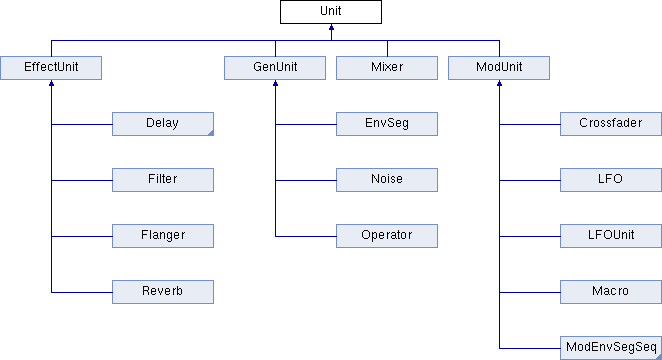
\includegraphics[scale=0.5]{img/unit-inherit}
  \caption{The inheritance diagram of the Unit class. GenUnits are Units that generate samples. EffectUnits apply some effect to a sample, e.g. a sample delay.}
  \label{fig:unit-inherit}
\end{figure}

\footnotetext{In C++, a pure virtual function is a function that does not have any standard implementation and thus requires the derived classes of the class that declares the pure virtual function to implement that function on their own. A class that declares a pure virtual method is termed an \emph{abstract} class and may not be instantiated.}

\subsubsection{The \texttt{modulate} method}

All classes derived from the ModUnit class must implement the \texttt{modulate} method, which takes the sample to modulate, a depth value between 0 (no modulation) and 1 (full modulation) as well as a maximum boundary as its arguments. In the case of LFOs, the maximum boundary parameter determines the value that is added to the sample. For example, when the amplitude of a unit is modulated, the maximum boundary is 1, meaning that the value added to the sample is in the range of $[-A_{LFO} \cdot 1; A_{LFO} \cdot 1]$, whereas for the rate parameter of Envelope segments, where the maximum boundary is 10, the range is $[-A_{LFO} \cdot 10; A_{LFO} \cdot 10]$. The declaration of the \texttt{modulate} method in the ModUnit class is given below.

\begin{lstlisting}
  virtual double modulate(double sample, double depth, double maximum) = 0;
\end{lstlisting}

\noindent This method was the main motivation behind the creation of the ModUnit class and is especially important for ModDocks, as it makes it possible to polymorphically access the \texttt{modulate} method of any ModUnit through a pointer-to-ModUnit (\texttt{ModUnit*}). This means that each ModUnit can have its own definition of what it means to modulate a sample. Table \ref{code:modlfo} shows the definition of the \texttt{modulate} method in the LFO and Table \ref{code:modenv} in the Envelope class.

\begin{table}[ht!]
  \code{modlfo.cpp}
  \caption{The implementation of the \texttt{modulate} method for LFOs.}
  \label{code:modlfo}
\end{table}

\begin{table}
  \code{modenv.cpp}
  \caption{The implementation of the \texttt{modulate} method for Envelopes. Note that for the Envelope class, the paramter \texttt{maximum} is not relevant, which is why it is never used. This shows that all that matters is that the method returns a modulated sample --- what "modulate" means is up to the class that implements it.}
  \label{code:modenv}
\end{table}

\subsubsection{ModDocks}

A ModDock is simply a collection of ModUnits. The ModDock collects all the modulated samples of individual ModUnits in the dock and returns an average over all samples. For example, if one LFO adds a value of $0.3$ to the amplitude parameter of a Unit with a current amplitude of $0.5$ and another subtracts a value of $0.1$, the final amplitude of that Unit will be $0.6$, as $\frac{(0.5 + 0.3) + (0.5 - 0.1)}{2} = 0.6$. Moreover, this means that if the two LFOs were to add/subtract the same absolute value but with a different sign, for example $-0.4$ and $0.4$, the net difference would be $0$ and the amplitude would remain $0.5$. Something else the ModDock takes care of is boundary checking and value adjustment. This means that, continuing the example given above, were an LFO to add a value of $±1$ to the base amplitude of $0.5$, the amplitude would not oscillate in the range $[-1.5;1.5]$. Rather, the ModDock ensures that the value trespasses neither the maximum boundary nor the minimum boundary, which is another parameter supplied to the ModDock. Therefore, the amplitude value would remain in the optimal range of $[-1;1]$. Alongside the maximum and the minimum boundary, the Unit who owns the ModDock can pass the current base value of the parameter to be modulated to the ModDock. In the aforementioned example, the base value would be $0.5$. Also, the ModDock can store the depth of modulation of individual ModUnits. Because both the \texttt{depth} and the \texttt{maximum} parameter of the \texttt{modulate} method for ModUnits are now stored in an instance of the \texttt{ModDock} class, the \texttt{modulate} method has a much simpler declaration in the \texttt{ModDock} class:

\begin{lstlisting}
  double modulate(double sample);
\end{lstlisting}

\noindent What this simplification of the \texttt{modulate} method requires, however, is that the maximum and minimum boundary as well as an initial base value are passed to the relevant ModDock in the construction of the Unit that owns it. Additionally, the ModDock must be notified whenever the base value changes. Table \ref{code:moddockconst} shows how these parameters may be passed to a ModDock and updated when necessary.

\begin{table}[ht!]
  \code{moddockconst.cpp}
  \caption{}
  \label{code:moddockconst}
\end{table}

\pagebreak

\subsubsection{Sidechaining}

One of the most interesting and equally complicated tasks encountered when creating the ModDock system was the implementation of side-chaining. Side-chaining makes it possible to have one ModUnit in a ModDock modulate the depth parameter of another ModUnit in that same ModDock. Borrowing from the terminology of digital communication, a ModUnit that side-chains another ModUnit is termed a "Master" and the ModUnit being side-chained is called a "Slave". Moreover, it was decided that any ModUnit that is not a Master shall be called a non-Master. A non-Master is any ModUnit that is either a Slave or not involved in any side-chaining relationship at all --- a normal ModUnit. It should be noted that the signal of a Master does not affect the final modulation value of a ModDock directly, i.e. the modulation value of a Master is not taken into consideration during the averaging process described above, but only indirectly, by modulating the depth of a Slave. Therefore, a ModUnit can be either a Master and contribute to the final modulation directly or be a non-Master and contribute to the final value directly. It should be noted that it is entirely possible to have one Master modulate multiple Slaves and for one Slave to have multiple Masters. Figure \ref{fig:flowsc} depicts these relationships in a flow-chart. Figure \ref{fig:scsketch} shows a scan of early sketches created while implementing side-chaining.\\

\noindent What Figure \ref{fig:scsketch} also displays is that there are two possible ways to implement side-chaining. The first method, which was ultimately not chosen, is to have each ModUnit in the ModDock have its own ModDock where Masters could be inserted. The second method involves internally linking Masters and Slaves within the ModDock. This second implementation was finally decided to be the better one as it does not require the instantiation of a full new ModDock for each ModUnit while providing the same functionality. Listing \ref{code:moditem} shows all private members of the \texttt{ModDock} class. Special attention should be payed to the \texttt{ModItem} struct, which is essential to the implementation of side-chaining and is very similar to the concept of a Linked-List. Each \texttt{ModItem} stores the aforementioned pointer-to-ModUnit to access the \texttt{modulate} method of the ModUnit. Moreover, there is one vector of indices for all Masters of that particular ModItem and one vector of indices for all of its Slaves. These indices refer to the positions of Masters/Slaves in the vector where all ModItems are stored, the \texttt{modItems\_} vector. When the user sets up a side-chain relationship between two ModItems of a ModDock, the index of the Slave is added to the Slave vector of the Master and the index of the Master is inserted into the Master vector of the Slave. Should the user wish to "un-side-chain" two ModItems, their indices are removed from the each other's appropriate vector.\\

\noindent Moreover, the \texttt{ModItem} struct holds a baseDepth variable. This variable is similar to the baseValue of the ModDock, in the sense that is the ModItem's original depth which serves as the base value for modulation by other ModItems. The modulation of a Slave by its Masters is implemented in the exact same way that a parameter of a Unit is modulated by a ModDock's ModUnits. Modulated Slave samples are summed and averaged over their number. Listing \ref{code:moddockmodulate} gives the full definition of the \texttt{modulate} method of the ModDock class. In lines 9 to 35, Slaves are modulated by their Masters. Subsequently, in lines 39 to 62, the sample passed to the function from the Unit who owns the ModDock is modulated by all non-Masters and finally returned.

\begin{figure}[p!]
  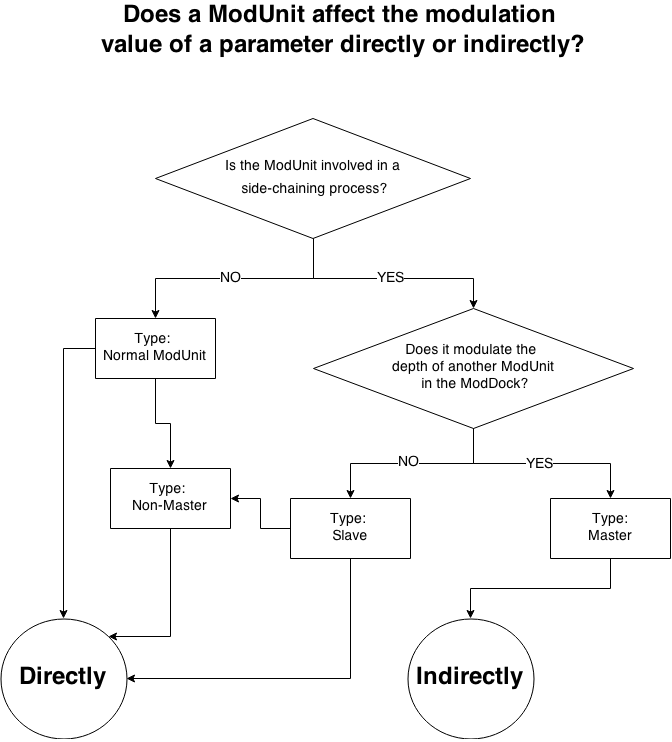
\includegraphics[scale=0.7]{img/flowsc}
  \caption{}
  \label{fig:flowsc}
\end{figure}

\begin{figure}[p!]
  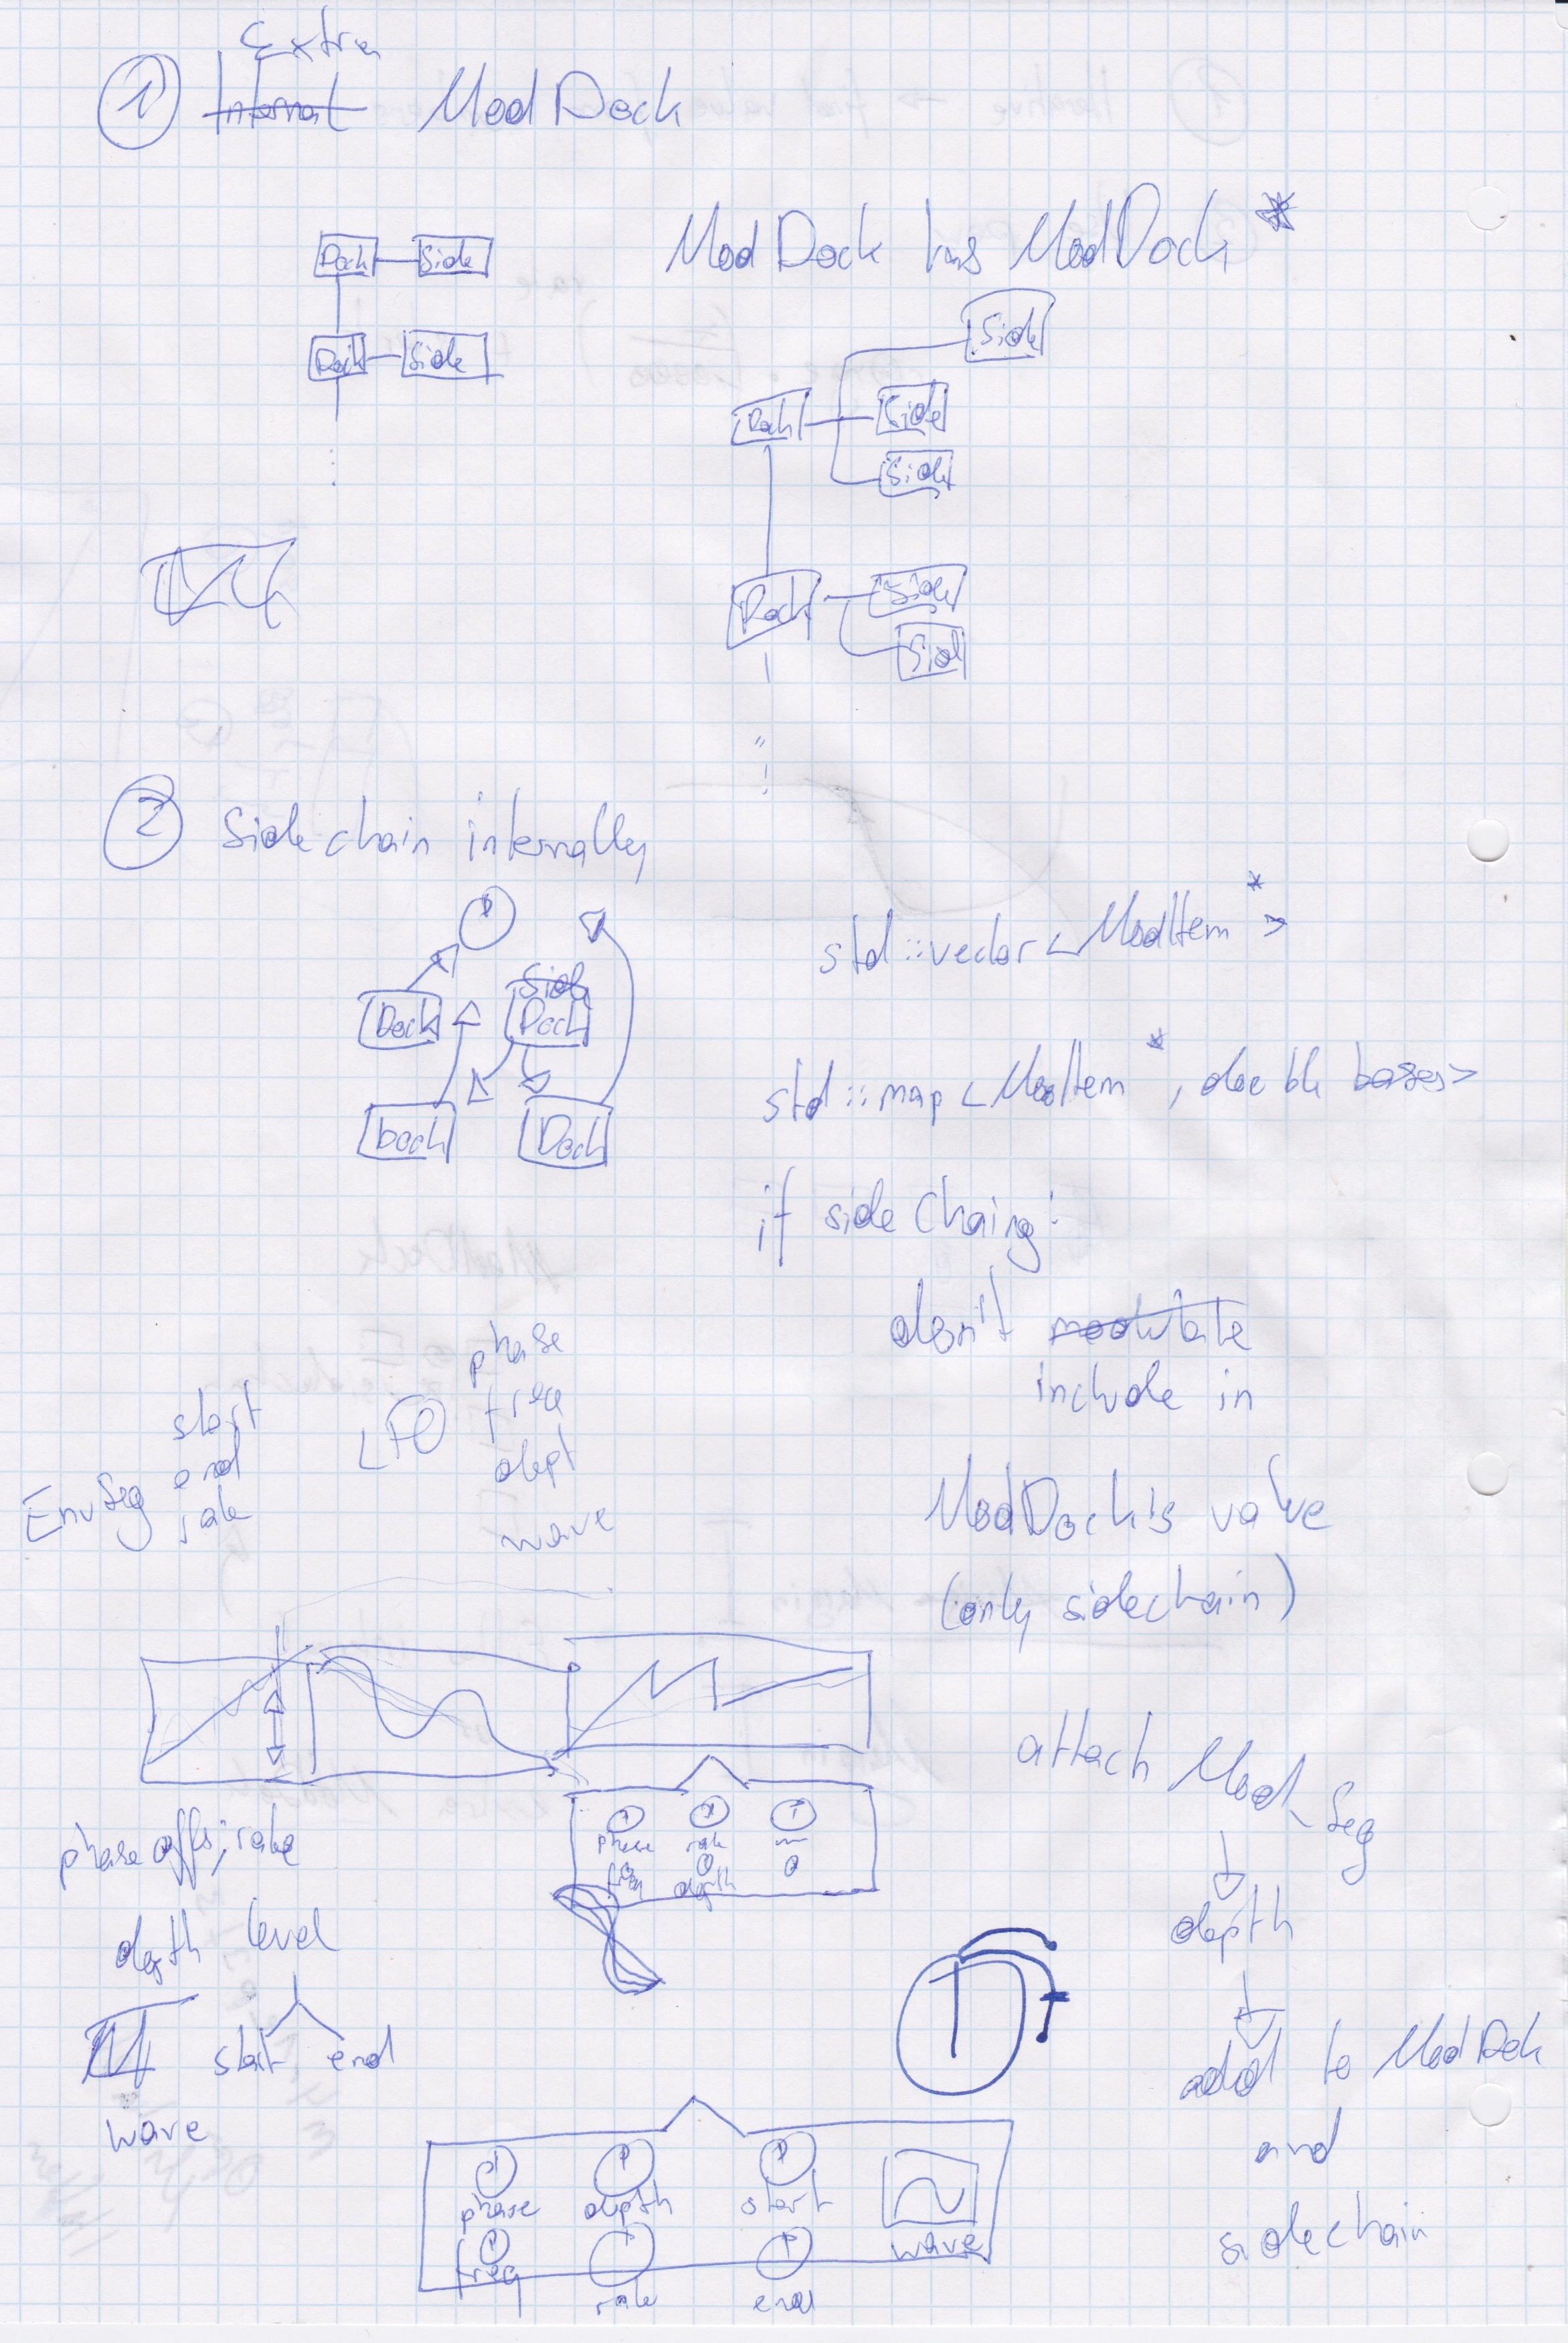
\includegraphics[scale=0.8]{img/scsketch}
  \caption{}
  \label{fig:scsketch}
\end{figure}

\pagebreak

\chapter{Crossfading Sound}

In digital music, it is often useful to crossfade or "mix" between two signals\footnotemark{}. When two signals $A$ and $B$ are used to produce a new signal $C$, crossfading means to control the amount by which signal $C$ is composed of signal $B$ in dependence of the amount by which it is composed of signal $A$. This is especially interesting when the two signals stem from ModUnits, making it possible to mix between their modulation signals. This idea lead to the creation of the \texttt{Crossfader} class, which is itself a ModUnit and will be described in this section. Equation \ref{eq:lcrossfade1} defines the concept of crossfading, in its most basic form, mathematically.

\begin{equation}
  C(t) = (A(t) \cdot x) + (B(t) \cdot (1 - x)), \text{where } x \in [0;1]
  \label{eq:lcrossfade1}
\end{equation}

\footnotetext{Crossfading is most commonly known as the technique a DJ may use to mix between two pieces of music during his/her performance.}

The following sections will examine three techniques of crossfading as described by Daniel R. Mitchell in his book \emph{BasicSynth: Creating a Music Synthesizer in Software}, pages 96 to 99. Additionally, their implementation in C++ will be outlined.

\section{Linear Crossfading}

Linear crossfading is the simplest form of crossfading. Its mathematical definition was already given in Equation \ref{eq:lcrossfade1}, showing that the crossfade value for the "right" signal, $B$, is indirectly proportional to the value for the "left" signal, $A$. This means that when the left value increases, the right value decreases and vice-versa. It should be noted that it is common to provide a range of $[-1;1]$ or $[-100;100]$ (preferred) instead of the mathematically easier range of $[0;1]$, simply to make the interaction more intuitive to the user. Therefore, Equation \ref{eq:lcrossfade1} must be re-formed to Equation \ref{eq:lcrossfade2}. Table \ref{tb:lcrossfade} shows crossfade values alongside the resulting multipliers for signals $A$ and $B$.

\begin{equation}
  C(t) = (A(t) \cdot \frac{100 - x}{200}) + (B(t) \cdot \frac{100 + x}{200}), \text{where } x \in [-100;100]
  \label{eq:lcrossfade2}
\end{equation}

\begin{table}[h!]

  \centering

  \begin{tabular}[]{| l | l | l |}
    \hline
    \rowcolor[gray]{0.8}
    Value & Multiplier $A$ & Multiplier $B$ \\\hline
    -100 & 1 & 0\\\hline
    -75 & 0.875 & 0.125\\\hline
    -50 & 0.75 & 0.25\\\hline
    -25 & 0.625 & 0.375\\\hline
    0 & 0.5 & 0.5\\\hline
    25 & 0.375 & 0.625\\\hline
    50 & 0.25 & 0.75\\\hline
    75 & 0.125 & 0.875\\\hline
    100 & 0 & 1\\
    \hline
  \end{tabular}

  \caption{Crossfade values alongside the resulting multipliers for signals $A$ and $B$.}

  \label{tb:lcrossfade}

\end{table}

\section{Crossfading with the $\sin$ function}

Another technique of crossfading involves the use of the $\sin$ function to compute the multipliers for signals $A$ and $B$. This is said to improve the "smoothness" of the mix \citebs{98}. Because the $\sin$ function operates with radians, the crossfade values from Equation \ref{eq:lcrossfade2} must be multiplied with $\frac{\pi}{2}$, leading to Equation \ref{eq:scrossfade} for cross-fading with the $\sin$ function. It should be noted that the center value for this technique is not $0.5$, but $\frac{\sqrt{2}}{2}$ or $\sin(\frac{\pi}{4})$. Table \ref{tb:scrossfade} gives cross-fade values using the $\sin$ function and the multipliers that result from them. Figure \ref{fig:lscrossfade} shows how this method of crossfading compares to linear crossfading in a coordinate system.

\begin{equation}
  C(t) = (A(t) \cdot \sin(\frac{100 - x}{200} \cdot \frac{\pi}{2})) + (B(t) \cdot \sin(\frac{100 + x}{200} \cdot \frac{\pi}{2})), \text{where } x \in [-100;100]
  \label{eq:scrossfade}
\end{equation}

\begin{table}[h!]

  \centering

  \begin{tabular}[]{| l | l | l |}
    \hline
    \rowcolor[gray]{0.8}
    Value & Multiplier $A$ & Multiplier $B$ \\\hline
    -100 & 1 & 0\\\hline
    -75 & 0.980 & 0.195\\\hline
    -50 & 0.924 & 0.383\\\hline
    -25 & 0.831 & 0.556\\\hline
    0 & 0.707 & 0.707\\\hline
    25 & 0.556 & 0.831\\\hline
    50 & 0.383 & 0.924\\\hline
    75 & 0.195 & 0.980\\\hline
    100 & 0 & 1\\
    \hline
  \end{tabular}

  \caption{Crossfade values when using the $\sin$ function, alongside the resulting multipliers for signals $A$ and $B$.}

  \label{tb:scrossfade}

\end{table}

\begin{figure}[p!]

  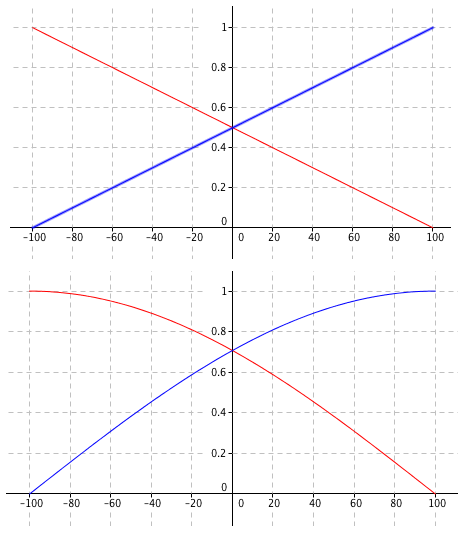
\includegraphics[scale=0.7]{img/lscrossfade}

  \caption{The top graph depicts linear crossfading and the bottom graph crossfading with the $\sin$ function. The red line is the multiplier for signal $A$ and the blue line is the multiplier for signal $B$.}

  \label{fig:lscrossfade}

\end{figure}

\section{Radical Crossfading}

Another method of non-linear crossfading involves the computation of signal multipliers according to a square-root function. Similar to crossfading with the $\sin$ function, values do not always add up to $1$ for radical crossfading. Moreover, the middle value is again $\frac{\sqrt{2}}{2}$ or $\sin(\frac{\pi}{4})$. Equation \ref{eq:sqrtcrossfade} shows the appropriate mathematical definition for radical crossfading and Table \ref{tb:sqrtcrossfade} displays crossfade values alongside resultant multipliers. Additionally, Figure \ref{fig:sqrtcrossfade} puts radical crossfading into a coordinate-system.

\begin{equation}
  C(t) = (A(t) \cdot \sqrt{\frac{100 - x}{200}}) + (B(t) \cdot \sqrt{\frac{100 + x}{200}}), \text{where } x \in [-100;100]
  \label{eq:sqrtcrossfade}
\end{equation}

\begin{table}[ht!]

  \centering

  \begin{tabular}[]{| l | l | l |}
    \hline
    \rowcolor[gray]{0.8}
    Value & Multiplier $A$ & Multiplier $B$ \\\hline
    -100 & 1 & 0\\\hline
    -75 & 0.935 & 0.354\\\hline
    -50 & 0.866 & 0.500\\\hline
    -25 & 0.791 & 0.612\\\hline
    0 & 0.707 & 0.707\\\hline
    25 & 0.612 & 0.791\\\hline
    50 & 0.500 & 0.866\\\hline
    75 & 0.354 & 0.935\\\hline
    100 & 0 & 1\\
    \hline
  \end{tabular}

  \caption{Radical crossfade values with resultant multipliers for signals $A$ and $B$.}

  \label{tb:sqrtcrossfade}

\end{table}

\begin{figure}[h!]

  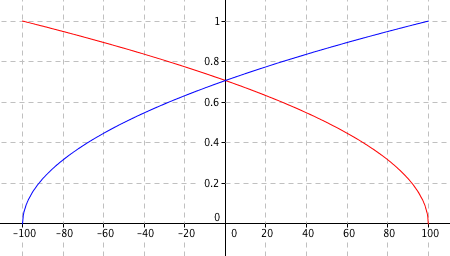
\includegraphics[scale=0.7]{img/sqrtcrossfade}

  \caption{Radical crossfading shown in a coordinate-system. The red line is the multiplier for signal $A$ and the blue line is the multiplier for signal $B$.}

  \label{fig:sqrtcrossfade}

\end{figure}

\pagebreak

\section{Scaling Crossfade values}

It is possible to scale crossfade values resulting from radical crossfading as well as from crossfading with the $\sin$ function in such way that the multipliers at the center crossfade value are again both $0.5$ instead of $\frac{\sqrt{2}}{2}$. To do so, one simply needs to multiply all multipliers by $\frac{\sqrt{2}}{2}$, since $(\frac{\sqrt{2}}{2})^2 = 0.5$. This leads to Equations \ref{eq:scrossfadesc}, for crossfading with the $\sin$ function, and \ref{eq:sqrtcrossfadesc}, for radical crossfading as well as Tables \ref{eq:scrossfadesc} and \ref{eq:sqrtcrossfadesc} for respective multipliers. One caveat of scaling is that all values become smaller.

\begin{equation}
  C(t) = (A(t) \cdot \sin(\frac{100 - x}{200} \cdot \frac{\pi}{2}) \cdot \frac{\sqrt{2}}{2}) + (B(t) \cdot \sin(\frac{100 + x}{200} \cdot \frac{\pi}{2}) \cdot \frac{\sqrt{2}}{2}), \text{where } x \in [-100;100]
  \label{eq:scrossfadesc}
\end{equation}

\begin{equation}
  C(t) = (A(t) \cdot \sqrt{\frac{100 - x}{200}} \cdot \frac{\sqrt{2}}{2}) + (B(t) \cdot \sqrt{\frac{100 + x}{200}} \cdot \frac{\sqrt{2}}{2}), \text{where } x \in [-100;100]
  \label{eq:sqrtcrossfadesc}
\end{equation}

\begin{table}[h!]

  \centering

  \begin{tabular}[]{| l | l | l |}
    \hline
    \rowcolor[gray]{0.8}
    Value & Multiplier $A$ & Multiplier $B$ \\\hline
    -100 & 0.707 & 0\\\hline
    -75 & 0.694 & 0.138\\\hline
    -50 & 0.653 & 0.270\\\hline
    -25 & 0.588 & 0.393\\\hline
    0 & 0.5 & 0.5\\\hline
    25 & 0.393 & 0.588\\\hline
    50 & 0.270 & 0.653\\\hline
    75 & 0.138 & 0.694\\\hline
    100 & 0 & 0.707\\
    \hline
  \end{tabular}

  \caption{Scaled values for crossfading with the $\sin$ function, alongside the resulting multipliers for signals $A$ and $B$.}

  \label{tb:scrossfadesc}

\end{table}

\begin{table}[ht!]

  \centering

  \begin{tabular}[]{| l | l | l |}
    \hline
    \rowcolor[gray]{0.8}
    Value & Multiplier $A$ & Multiplier $B$ \\\hline
    -100 & 0.707 & 0\\\hline
    -75 & 0.661 & 0.25\\\hline
    -50 & 0.612 & 0.354\\\hline
    -25 & 0.559 & 0.433\\\hline
    0 & 0.5 & 0.5\\\hline
    25 & 0.433 & 0.559\\\hline
    50 & 0.354 & 0.612\\\hline
    75 & 0.25 & 0.661\\\hline
    100 & 0 & 0.707\\
    \hline
  \end{tabular}

  \caption{Scaled radical crossfade values with resultant multipliers for signals $A$ and $B$.}

  \label{tb:sqrtcrossfade}

\end{table}

\section{Creating Crossfade Tables}

Because crossfade values are constant, i.e. there is only one possible tuple of multipliers for each crossfade value, it was decided that these multipliers should be stored in a table once and then looked-up. This is a lot more efficient than having to calculate each multiplier at every request. Similar to Wavetables, these crossfade tables are written to a file and then written into computer memory at program start-up. The only difference between Wavetable files and crossfade table files is that the former are stored in binary and the latter in plain-text, as the the size of crossfade tables is only 201 instead of 4096, the size of a Wavetable. Table \ref{code:crossfadetables} shows a computer program, this time written in Python, to compute and store crossfade tables.

\begin{table}[hbt!]
  \lstinputlisting[language=Python]{code/crossfadetables.py}
  \caption{}
  \label{code:crossfadetables}
\end{table}

\chapter{Filtering Sound}

A feature any digital synthesizer should include is the possibility to filter sound. In digital signal processing (DSP) and more specifically in audio processing, to filter a signal means to "alter [its] frequency spectrum [...] by amplifying or attenuating selected frequencies". \citebs{102}.\\

\noindent The discussion of digital filters is closely linked to the concept of a signal's phase and how the phase relationship between two \emph{input} signals influences the properties of the \emph{output} signal produced when the two input signals interact and interfere either constructively or destructively. A simple examples of phase relationships from the analog realm is the situation where signals $A$ and $B$ are exactly identical and consequently have a phase difference $\Delta \phi$of $0$. If these signals are summed, the resulting signal $C$ will have an amplitude twice as high or low as that of signal $A$ or $B$ in every single point of its signal --- the input signals interfere \emph{constructively}. Conversely, if signals $A$ and $B$ have a phase shift of 180\degree or $\pi$ radians, the two signals interefere \emph{destructively} and result in signal $C$ having a constant amplitude of exactly $0$, as the amplitude values of signals $A$ and $B$ cancel each other out in each point of the signal.\\

\noindent In digital systems, where signals are represented discretely, i.e. with periodically recorded samples, this behaviour can be modeled by applying a \emph{sample delay}. \citebs{103} For example, if a signal that is periodically represented by 10 samples is summed with a version of itself that is delayed by 5 samples, that version will effectively be phase-shifted by 180\degree and thus the summation of these two signals will result in silence. Had only one sample been delayed instead of five, the phase difference $\Delta \phi$ would have only been 36\degree or $\frac{2\pi}{10}$ radians --- one tenth of a period. The amount of phase difference $\Delta \phi$ depends on both the number of samples a signal is represented by, so the sample rate of the system, and the number of samples that are delayed. An equation to calculate the phase difference in radians, given these parameters, is shown in Equation \ref{eq:phasediff}, where $f$ is the frequency of the signal, $f_{s}$ the sample rate and $N$ the number of samples delayed. If $2\pi$ is replaced by 360, this Equation yields the same phase difference in degrees.\\

\begin{equation}
  \Delta\phi = \frac{N \cdot f}{f_{s}} \cdot 2\pi
  \label{eq:phasediff}
\end{equation}

\noindent From Equation \ref{eq:phasediff} it can be deduced that a sample delay causes different phase relationships for different frequencies of the original signal. To give an example: let one sample be delayed in a system with a sample rate $f_{s}$ equal to 20 kHz. In such a system, a signal with a frequency of 1 Hz is represented by 20000 samples. Consequently, summing such a signal with a version of itself delayed by one sample would make the resulting, filtered signal almost twice as loud, as $\Delta\phi$ is only about 0.018\degree. However, a signal with the maximum possible frequency of 10 Khz (the Nyquist limit) is represented by only 2 samples. Therefore, delaying one sample equals a phase shift of 180\degree, which results in silence when the signal is summed with the delayed version of itself. This introduces the concept of a filter's \emph{frequency response}, which describes how a filter influences a signal's frequency spectrum. For the filter just described, the frequency response would look approximately like Figure \ref{fig:freqresp}.\\

\begin{figure}
  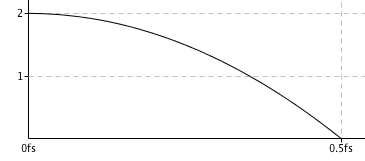
\includegraphics[scale=0.8]{img/freqresp}
  \caption{The frequency response of a one-sample-delay filter. The most constructive interference is at 0 Hz, a signal that is constant with $f(t) = 1$. Such a signal with a frequency of 0 Hz is also called DC, for direct current, because in analog circuits a DC current is constant. The most destructive interference occurs at $\frac{f_{s}}{2}$ Hz.}
  \label{fig:freqresp}
\end{figure}

\noindent One way to change the frequency response of a filter is to weight samples of the input signal as well as the delayed samples with \emph{filter coefficients} \citebs{105, 110}. Whereas previously a one-sample delay could be modeled by Equation \ref{eq:onedelay1} \citebs{104}, where $y_{n}$ is the output, $x_{n}$ the current and $x_{n-1}$ the delayed sample, Equation \ref{eq:onedelay2} \citebs{103}, where $a$ and $b$ are the respective filter coefficients, must be used when samples are weighted with coefficients. Visually, such a one-sample delay can be represented with the diagram shown in Figure \ref{fig:onedelay}.

\begin{equation}
  y_{n} = x_{n} + x_{n-1}
  \label{eq:onedelay1}
\end{equation}

\begin{equation}
  y_{n} = bx_{n} + ax_{n-1}
  \label{eq:onedelay2}
\end{equation}

\begin{figure}[h!]
  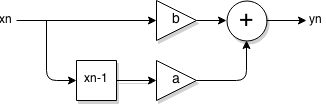
\includegraphics[scale=0.8]{img/onedelay}
  \caption{A one-sample delay with filter coefficients $a$ and $b$. Triangles are amplifiers/attenuators. Samples are summed at the circle with the + at its center.}
  \label{fig:onedelay}
\end{figure}

\pagebreak

\section{FIR and IIR Filters}

\noindent While a filter's frequency response describes how the frequency content of a signal is affected by that filter, its influence on a signal in the time domain is given by the filter's \emph{impulse response} or \emph{kernel}. More precisely, an impulse response determines what a filter outputs when its input is a delta function, $\delta$, which has a normalized \emph{impulse}, meaning a sample with an amplitude of 1, as its first sample while all other subsequent samples have an amplitude of 0. The $\delta$ function is also referred to as the \emph{unit impulse}. \citedsp{108} For example, if the filter coefficients of the three-sample delay filter shown in Figure \ref{fig:threedelay} are all equal to 0.5 ($a = b = c = 0.5$), leading to Equation \ref{eq:threedelay}, then Figure \ref{fig:impresp} gives the impulse response of this filter when it is fed the $\delta$ function depicted in Figure \ref{fig:deltafunc}. What this impulse response shows is that if a sample $x_{n}$ with an amplitude of 1 is input into this filter, the first sample output will be $1 + \frac{0}{2}+ \frac{0}{2}+ \frac{0}{2} = 1$. The second sample to exit this filter will then be $0 + \frac{1}{2}+ \frac{0}{2}+ \frac{0}{2} = 0.5$, where, following the definition of the $\delta$ function given above, the new $x_{n}$ is equal to 0, while the previous $x_{n}$ that was equal to 1 has moved into the position of $x_{n-1}$. The third sample will be equal to $0 + \frac{0}{2} + \frac{0.5}{2}+ \frac{0}{2} = 0.25$ and finally the fourth sample has a value of $\frac{1}{8}$.

\begin{equation}
  y_{n} = x_{n} + \frac{x_{n-1}}{2}+ \frac{x_{n-2}}{2}+ \frac{x_{n-3}}{2}
  \label{eq:threedelay}
\end{equation}

\begin{figure}
  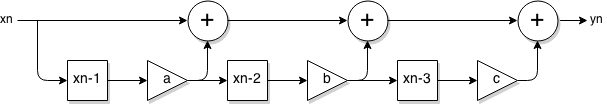
\includegraphics[scale=0.7]{img/threedelay}
  \caption{A three-sample delay filter.}
  \label{fig:threedelay}
\end{figure}

\begin{figure}

  \TopFloatBoxes

  \begin{floatrow}

    \ffigbox{\caption{A delta function, also called a unit impulse. The first sample has an amplitude of 1 while all other samples are equal to 0.} \label{fig:deltafunc}}{ 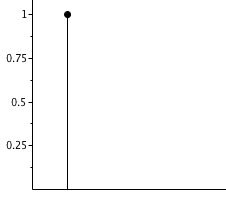
\includegraphics[scale=0.7]{img/deltafunc}}

    \ffigbox{\caption{The impulse response of the three-sample delay filter depicted in Figure \ref{fig:threedelay}.} \label{fig:impresp}}{ 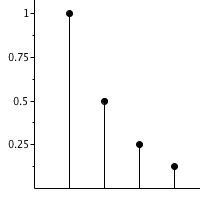
\includegraphics[scale=0.7]{img/impresp}}

  \end{floatrow}

\end{figure}

\noindent The operation that was just performed on the $\delta$ function is called "convolution". Convolution has its own mathematical symbol: $\ast$. To convolve a signal means to apply an impulse response to every of its samples. Table \ref{code:convolve} shows a C++ program to perform convolution (based on pseudo-code cf. Mitchell, 2008, p. 107).\\

\begin{table}
  \code{convolve.cpp}
  \caption{A C++ function to convolve a signal vector with an impulse response vector. It should be noted that to convolve a signal vector of size $m$ with an impulse response vector of size $n$, the output vector must have a minimum size of $m + (n - 1)$.}
  \label{code:convolve}
\end{table}

\noindent The filters described so far are called Finite Impulse Response (FIR) filters, because their impulse response is of finite size, like the one shown in Figure \ref{fig:impresp}, caused by the Filter depicted in Figure \ref{fig:threedelay}. Given that in this three-sample delay filter all filter coefficients have the same value of $0.5$, the diagram could actually be re-arranged and simplified if the three delays are replaced by a single \emph{recursive} delay. Instead of processing an input sample, a recursive delay is fed an output sample, which it then amplifies or attenuates and feeds back into the signal. This re-arranged filter, also called a \emph{feedback loop}, is shown in Figure \ref{fig:iirdelay}. Because this feedback loop could theoretically go on forever, such a filter is called an Infinite Impulse Response (IIR) filter. Equation \ref{eq:iirdelay} gives a mathematical definition for the filter shown in Figure \ref{fig:iirdelay}. To prove that this filter results in the same response as the FIR filter from before, it can be fed a $\delta$ function. Because $y_{n-1}$ is initially 0, the first output $y_{n}$ will simply be $1 + \frac{0}{2}$. For the second sample, $y_{n-1}$ takes on the value of the previous output, which was 1. Therefore, the second output sample is $0 + \frac{1}{2} = 0.5$, the next sample $0 + \frac{0.5}{2}$ and so on. Because this is an IIR filter, this process could theoretically go on ad infinitum. $x_{n}$ is equal to 0 for all samples other than the first because of the way the $\delta$ function is defined.

\begin{equation}
  y_{n} = x_{n} + \frac{y_{n-1}}{2}
  \label{eq:iirdelay}
\end{equation}

\begin{figure}
  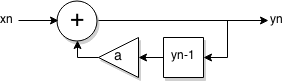
\includegraphics[scale=0.7]{img/iirdelay}
  \caption{An IIR delay filter.}
  \label{fig:iirdelay}
\end{figure}

\pagebreak

\section{Bi-Quad Filters}

A common arrangement of FIR and IIR filters is a so-called bi-quad filter. A "bi-quad filter combines one and two sample feedforward delays (FIR) with one and two sample feedback delays (IIR)" \citebs{109}. Figure \ref{fig:biquad} shows such a bi-quad filter. The Equation to calculate the sample output of a bi-quad filter is given by Equation \ref{eq:biquad}.

\begin{figure}[h!]
  \includegraphics[scale=0.7]{img/biquad}
  \caption{A bi-quad filter in direct form II. In direct form I, the filter is turned inside-out. The result is the same, however direct form II is a little more concise to implement. }
  \label{fig:biquad}
\end{figure}

\begin{equation}
  y_{n} = b_{0}(x_{n} - a_{1}y_{n-1} - a_{2}y_{n-2}) + b_{1}x_{n-1} + b_{2}x_{n-2}
  \label{eq:biquad}
\end{equation}

\subsection{Implementation}

In the synthesizer created for this thesis, the \texttt{Filter} class implements a bi-quad filter. Table \ref{code:filter} shows the \texttt{Filter} class' \texttt{process} method, which takes an input sample and returns a filtered output sample.

\begin{table}[h!]
  \code{filter.cpp}
  \caption{C++ function to filter an input sample and return an output sample. This function implements the bi-quad filter equation given by Equation \ref{eq:biquad}.}
  \label{code:filter}
\end{table}

\pagebreak

\section{Filter Types}

Bi-quad filters can be used to create a variety of different filter types and corresponding frequency responses, simply by adjusting the filter's coefficients. When examining a frequency response, the term \textbf{passband} is used for the frequency range that should ideally not be affected by the filter. Conversely, the \textbf{stopband} are those frequency components the filter should, ideally, silence completely. The frequency at which the transition from minimum to maximum attenuation occurs is called the \textbf{cutoff frequency} and is denoted by $f_{c}$. Because no filter is perfect, this transition usually does not happen precisely at the specified cutoff frequency. Rather, there is a certain \textbf{transition band}, which is the range of frequencies where the transition takes place. Within this transition band, the cutoff frequency is defined as the frequency component where the amplitude reaches $\frac{\sqrt{2}}{2}$ (0.707...) or -3dB in power\footnotemark. If the transition band is narrow, the filter is said to have a fast \textbf{roll-off}. If it is rather wide, the roll-off is said to be slow. \citedsp{268} Figure \ref{fig:filterterm} depicts a typical frequency response and labels the relevant bands and frequencies. It should be noted that bi-quad filters and IIR filters in general show quite slow roll-off.

\footnotetext{A signal's power is measured in decibels (dB), which is a logarithmic unit of measurement. 20dB equals an increase in amplitude by one order of magnitude ($\cdot 10$) and -20dB a decrease by one order of magnitude ($\cdot 0.1$).}

\begin{figure}[h!]
  \includegraphics[scale=0.7]{img/filterterm}
  \caption{The frequency response of a filter with a relatively fast roll-off.}
  \label{fig:filterterm}
\end{figure}

\pagebreak

\subsection{Low-Pass Filters}

Low-Pass filters have their passband in the lower frequency ranges and their stopband in the higher ranges. A visualization of a low-pass bi-quad filter's frequency response when applied to a white noise signal\footnotemark{} is given in Figure \ref{fig:filterterm}.

\begin{figure}[p!]
  \includegraphics[scale=0.6]{img/lowpass}
  \caption{The frequency response of a low-pass bi-quad filter where $f_{c} = 5000$ Hz.}
  \label{fig:lowpass}
\end{figure}

\footnotetext{A white noise signal is used here because it has a flat frequency spectrum when un-filtered.}

\subsection{High-Pass Filters}

A high-pass filter is a low-pass filter whose spectrum has either been \emph{inverted} (flipped top-for-bottom) or \emph{reversed} (flipped left-for-right) \citedsp{271}. As a consequence, high-pass filters let high frequencies pass, while stopping lower frequencies. Figure \ref{fig:highpass} shows an appropriate frequency response.

\begin{figure}[p!]
  \includegraphics[scale=0.6]{img/highpass}
  \caption{The frequency response of a high-pass bi-quad filter where $f_{c} = 10000$ Hz.}
  \label{fig:highpass}
\end{figure}

\subsection{Band-Pass Filters}

Band-pass filters let frequency components in a specific range, e.g. 3000 to 5000 Hz, pass, while stopping all other frequencies lower or higher than the range of the passband. Such a filter can be created by first sending a signal through a low-pass and then through a high-pass filter. The passband of the filter created will then be the range of frequencies where the passband of the high-pass filter intersects that of the low-pass filter, since all other ranges are in a stopband. Figure \ref{fig:bandpass} shows the frequency response of a band-pass filter.

\begin{figure}[p!]
  \includegraphics[scale=0.6]{img/bandpass}
  \caption{The frequency response of a band-pass bi-quad filter where $f_{c} = 10000$ Hz.}
  \label{fig:bandpass}
\end{figure}

\subsection{Band-Reject Filters}

A band-reject filter, often referred to as a "notch" filter, can be seen as the opposite of a band-pass filter. While a band-pass filter stops all frequencies except for those immediately around the cutoff frequency, a band-reject filter stops only the frequencies at the cutoff frequency and lets all others pass. Besides using the correct filter coefficients for a bi-quad filter, a band-reject filter can also be created by using a low-pass and a high-pass filter \emph{in parallel}. This involves copying a signal, then sending one copy of the original signal through a low-pass filter and the other copy through a high-pass filter. The final signal is the sum of the signal output by the high-pass filter and the signal output by the low-pass filter. Figure \ref{fig:bandreject} displays the frequency response of a band-reject filter.

\begin{figure}[p!]
  \includegraphics[scale=0.6]{img/bandreject}
  \caption{The frequency response of a band-reject bi-quad filter where $f_{c} = 10000$ Hz.}
  \label{fig:bandreject}
\end{figure}

\pagebreak

\subsection{All-Pass Filters}

A very special type of filter is the so-called all-pass filter. As its name implies, an all-pass filter lets all frequencies pass and stops none. What could possibly be the use of such a filter? The answer lies in the second alteration a filter performs on a signal: a change in phase. All-pass filters are used to change a signal's phase while leaving its amplitude un-altered at all frequencies.

\section{Filter Coefficients}

Let $\omega = \frac{2\pi f_{c}}{f_{s}}$ and $\alpha = \frac{\sin(\omega)}{2Q}$, where Q is the filter's \emph{Quality Factor}\footnotemark{}, then Table \ref{tb:coef} gives the values the various filter coefficients of a bi-quad filter must take on to achieve the wanted frequency response. These values were determined by Robert Bristow-Johnson from analog filter circuits \footnote{Source: \url{http://www.musicdsp.org/files/Audio-EQ-Cookbook.txt}}.

\footnotetext{The Quality Factor can be said to control to some extent the bandwith of a filter's transition band as well as the amplitude peak of the passband before transitioning to the stopband.}

\begin{table}[h!]

  \centering

  \renewcommand{\arraystretch}{3}
  \begin{tabular}[]{ | c | c | c | c | c | c |}
    \hline
    \rowcolor[gray]{0.8}
    Filter Type & $a_{1}$ & $a_{2}$ & $b_{0}$ & $b_{1}$ & $b_{2}$ \\
    \hline
    Low-Pass & $\frac{-2\cos(\omega)}{1 + \alpha}$ & $\frac{1 - \alpha}{1 + \alpha}$ & $\frac{1-\cos(\omega)}{2(1 + \alpha)}$ & $\frac{1-\cos(\omega)}{1 + \alpha}$ & $\frac{1-\cos(\omega)}{2(1 + \alpha)}$\\
    \hline
    High-Pass & $\frac{-2\cos(\omega)}{1 + \alpha}$ & $\frac{1 - \alpha}{1 + \alpha}$ & $\frac{1+\cos(\omega)}{2(1 + \alpha)}$ & $\frac{-(1+\cos(\omega))}{1 + \alpha}$ & $\frac{1+\cos(\omega)}{2(1 + \alpha)}$\\
    \hline
    Band-Pass & $\frac{-2\cos(\omega)}{1 + \alpha}$ & $\frac{1 - \alpha}{1 + \alpha}$ & $\frac{\sin(\omega)}{2(1 + \alpha)}$ & $0$ & $\frac{-\sin(\omega)}{2(1 + \alpha)}$\\
    \hline
    Band-Reject & $\frac{-2\cos(\omega)}{1 + \alpha}$ & $\frac{1 - \alpha}{1 + \alpha}$ & $\frac{1}{1 + \alpha}$ & $\frac{-2\cos(\omega)}{1 + \alpha}$ & $\frac{1}{1 + \alpha}$\\
    \hline
    All-Pass & $\frac{-2\cos(\omega)}{1 + \alpha}$ & $\frac{1 - \alpha}{1 + \alpha}$ & $\frac{1 - \alpha}{1 + \alpha}$ & $\frac{-2\cos(\omega)}{1 + \alpha}$ & $1$\\
    \hline
  \end{tabular}

  \caption{Filter coefficients for a bi-quad filter.}

  \label{tb:coef}

\end{table}


\chapter{Effects}

While the digital revolution made it possible to create popular effects like Echos, Flangers or Reverbs more efficiently using logic circuits and digital signal processing, most effects found in digital synthesizers today have a long history of analog implementation. Rock stars like Jimi Hendrix, famous for using the "Wah-Wah" effect, applied effects to their sound long before digitization. The following sections will describe four common effects and explain their implementation.

\section{Delay Lines and the Delay Effect}

Delay lines store samples and \emph{delay} their retrieval by a certain number of sample times. Just like delay lines are at the foundation of many digital filters, they are also the primary building block of a great number of different effects. Consequently, they must be examined and discussed thoroughly before attempting to create any other digital effects. However, having a well-founded understanding of delay lines also makes the implementation of many effects a trivial task. It should be noted that when a delay line is used as an effect simply to delay samples, it will be referred to as a "Delay" effect.

\subsection{Simple Delay Lines}

\noindent  If the time by which a sample is delayed is constant for each sample, a delay line can be implemented using a simple First-In-First-Out (FIFO) data-structure such as a Queue. Figure \ref{fig:simpledelay} visualizes such a delay line and Table \ref{code:simpledelay} shows a C++ implementation. \citebs{118}

\begin{figure}[h!]
  \includegraphics[scale=0.8]{img/simpledelay}
  \caption{Visualization of a simple FIFO delay line.}
  \label{fig:simpledelay}
\end{figure}

\begin{table}[t!]
  \code{simpledelay.cpp}
  \caption{A C++ class that implements a very simple delay line of fixed size.}
  \label{code:simpledelay}
\end{table}

\pagebreak

\subsection{Flexible Delay Lines}

While simple delay lines are easy to implement, they are not efficient if the delay time is not constant, as changing the size would require the re-allocation of memory to suit the new size and subsequent copying of all items from the old delay line into the new one. Moreover, the moving of all samples by one index after retrieving the latest output sample is highly inefficient, especially for long delay times. A more reasonable approach is to implement a delay line as a circular buffer with a fixed maximum length and then to vary the distance between a read and a write iterator relative to the current delay time. The circularity is achieved by wrapping the read or the write index back to the front of the buffer if either reaches the end. Figure \ref{fig:ringdelay} shows such a circular buffer in an abstract visualization, where the write iterator, which points to the position where incoming samples are stored into the delay line, is currently at index 0. The Figure also shows two possible positions of the read iterator, from which delayed samples are retrieved, which both result in a different delay time. It should be noted that read iterator A and B do not exist simultaneously, they just show possible indices for the read iterator. Read position A would cause a delay of 5 sample times while read position B would result in a 20 sample delay. Figure \ref{fig:seqdelay} shows the same buffer and iterators in a more realistic sequential layout, as it is stored in computer memory.

\begin{figure}[p!]
  \includegraphics[scale=0.7]{img/ringdelay}
  \caption{A circular delay buffer with two different possible read positions A and B. The labels inside the boxes are the relative sample delays and the labels outside the boxes are the sequential indices. The write iterator is where new samples are stored and the read iterators are where delayed samples are retrieved from.}
  \label{fig:ringdelay}
\end{figure}

\begin{figure}[p!]
  \includegraphics[scale=0.7]{img/seqdelay}
  \caption{The buffer from Figure \ref{fig:ringdelay} in a sequential layout.}
  \label{fig:seqdelay}
\end{figure}

\subsection{Interpolation}

It is also possible to have fractional delay values if samples are interpolated. Equation \ref{eq:interpolatedelay} shows how this interpolation process is performed, where $i$ is the integral and $f$ the fractional portion of the $n$-sample delay. Note that this is the same interpolation algorithm that is performed to retrieve sample values from fractional Wavetable indices.

\begin{equation}
  y_{n} = x_{i} + ((x_{i-1} - x_{i}) \cdot f)
  \label{eq:interpolatedelay}
\end{equation}

\subsection{Feedback and Decay}

Two parameters commonly associated with delay lines are \emph{feedback} and \emph{decay}. The feedback control of a delay line determines how much of the output signal is fed back into the delay line together with the input signal. The decay parameter determines the level of attenuation of the output signal as it leaves the delay line. It is "[...] applied each time the [fed-back] sample travels through the delay line and is equivalent to the dampening, or decay, of a signal over time". When these two parameters are used together, such a delay line is called a "Resonator". Figure \ref{fig:resonator} shows a block diagram for such a resonator and Figure \ref{fig:resonatorwav} displays a sound wave resulting from a resonator. \citebs{120}

\begin{figure}
  \includegraphics[scale=0.6]{img/resonatorwav}
  \caption{A sound wave resulting from a resonator. The initial silence is caused by the delay line filling up and delayed samples consequently still being equal to 0. The increase in amplitude per delay time (200 ms) is due to the feedback control. Because the decay is not 0, the amplitude does not double per delay time as it would if there were no decay and full feedback. Rather, the sound decays with time and would reach its maximum after 4 seconds.}
  \label{fig:resonatorwav}
\end{figure}

\begin{figure}
  \includegraphics[scale=0.7]{img/resonator}
  \caption{A resonating delay line.}
  \label{fig:resonator}
\end{figure}

\subsection{Dry/Wet Control}

Almost every effect, including the Delay effect, has what is called a "dry/wet" control. If the dry signal is the unchanged input signal and the wet signal the fully processed output signal, the dry/wet control determines how much of an effect is applied to the dry signal. Equation \ref{eq:drywet} gives a mathematical definition for this principle, where $dw$ is the dry/wet value between 0 (no effect) and 1 (full effect), $x_{n}$ the unchanged, "dry", input sample and $y_{n}$ the "wet" output signal from the effect.

\begin{equation}
  z_{n} = (x_{n} \cdot (1 - dw)) + (y_{n} \cdot dw)
  \label{eq:drywet}
\end{equation}

\subsection{Implementation}

In the synthesizer created for this thesis, a flexible delay line with all the properties and controls just mentioned is implemented in the \texttt{Delay} class. Relevant processing and updating methods of the \texttt{Delay} class are shown in Table \ref{code:delay}.

\begin{table}[thb!]
  \code{delay.cpp}
  \caption{Relevant member functions of the \texttt{Delay} class that implements a flexible delay line with feedback, decay, interpolation and dry/wet control.}
  \label{code:delay}
\end{table}

\pagebreak

\section{Echo}

The first effect that can be implemented very easily using just delay lines is the Echo effect. It is the result of summing an input sample with the output sample of a delay line. An implementation from the \texttt{Echo} class, derived from the \texttt{Delay} class, is shown in Table \ref{code:echo}.

\begin{table}[h!]
  \code{echo.cpp}
  \caption{The \texttt{process} method of the \texttt{Echo} class. This shows that an Echo is just the input sample summed with the output from the delay line.}
  \label{code:echo}
\end{table}

\section{Flanger}

A Flanger effect is created by mixing a signal with a delayed version of itself and varying the time by which it is delayed with a Low Frequency Oscillator. The middle delay time around which the LFO oscillates is called the "center" value. The term "depth" is used for the value that is added to or subtracted from the center value periodically. For example, if the center value is 10 ms and the depth 4 ms, the delay time will oscillate between 6 ms and 14 ms. The "rate" parameter controls how fast the LFO oscillates. A Flanger's "feedback" control is not the same as for delay lines, as it does not control how much of the output signal is fed back into the delay line. Rather, the feedback value determines how much of the sample at the center delay value is subtracted from the input sample. Varying the feedback controls the coloration and brightness of the sound produced. Lastly, a Flanger also has a dry/wet parameter, whose function was already described. Figure \ref{fig:flanger} depicts a block diagram for a Flanger. The sound produced by a Flanger effect can be described as a "swooshing" sound. \citebs{136} Table \ref{code:flanger} shows the \texttt{Flanger} class' \texttt{process} method.

\begin{figure}[p!]
  \includegraphics[scale=0.7]{img/flanger}
  \caption{Block diagram for a Flanger effect. The LFO controls the delay length. The feedback is negative because it is subtracted from the input sample. }
  \label{fig:flanger}
\end{figure}

\begin{table}[p!]
  \code{flanger.cpp}
  \caption{Member function of the \texttt{Flanger} class that implements flanging.}
  \label{code:flanger}
\end{table}

\section{Reverb}

When a musician plucks a string on his guitar or bangs a percussion drum in a closed room, the sound that reaches a listener's ears does not stem solely from the sound's source. Rather, the sound emited from the musical instrument reflects off the room's walls and ceiling as well as any other object it meets on the way to the listener. This mixture of original and reflectd sound is called reverberation \citebs{129}. Naturally, the degree of reverberation depends, among other things, to a large part on the space of the room in which the sound is emitted. For example, an organ will sound differently if played in a large cathedral than it will in a small classroom. Therefore, any parameters that control the degree of reverberation essentially determine the size of the "virtual room" in which the sound is played. Most reverberators, reverbs for short, allow the user to control the reverb "time" and the reverb "rate". The reverb time determines how long it takes for the sound to reach inaudible levels, while the reverb rate controls at what rate this fading out occurs. Finally, there is also a dry/wet control as for all other effects as well.

\subsection{Schroeder Reverb}

A relatively well-known and moderately popular reverb algorithm is the so-called "Schroeder Reverb", which consists of four parallel delay lines whose signals are fed into two all-pass filters connected in series. Figure \ref{fig:reverb} depicts a block diagram for a Schroeder Reverb. To simulate how sound waves reflect off different surfaces in a room, the delay lines are given different lengths. The decay parameter of these delay lines is determined by the reverb time and rate. The Schroeder Reverb's all-pass filters have fixed delay times and decay values. Table \ref{tb:reverb} gives these various delay line lengths and decay values. \citebs{133}

\begin{figure}[hb!]
  \includegraphics[scale=0.7]{img/reverb}
  \caption{Block diagram for a Schroeder Reverb effect.}
  \label{fig:reverb}
\end{figure}

\begin{table}[hb!]

  \centering

  \begin{tabular}[]{ | c | c | c |}
    \hline
    \rowcolor[gray]{0.8}
    Component & Delay Time & Decay Value \\\hline
    Delay A & 0.0297 & Variable\\\hline
    Delay B & 0.0371 & Variable \\\hline
    Delay C & 0.0411 & Variable \\\hline
    Delay D & 0.0437 & Variable \\\hline
    All-Pass A & 0.09638 & 0.0050 \\\hline
    All-Pass B & 0.03292 & 0.0017\\
    \hline
  \end{tabular}

  \caption{Delay times and decay values for a Schroeder Reverb.}

  \label{tb:reverb}

\end{table}

\pagebreak

\subsection{Implementation}

Table \ref{code:reverb} shows relevant member of function of the \texttt{Reverb} class, which implements a Schroeder Reverb.

\begin{table}[h!]
  \code{reverb.cpp}
  \caption{This code exerpt from the \texttt{Reverb} class shows how the Schroeder Reverb's delay lines and all-pass filters are initialized and then used to reveberate a signal.}
  \label{code:reverb}
\end{table}

\chapter{Synthesizing Sound}

The most important feature of a synthesizer is its capability to synthesize sound. Synthesizing sound means to combine two or more (audio) signals to produce a new signal. The many possibilities to synthesize sound waves with variable parameters enable musicians to create an uncountable number of different sounds. A synthesizer can be configured to resemble natural sounds such as that of wind or water waves, can emulate other instruments like pianos, guitars or bass drums and, finally, a synthesizer can also be used to produce entirely new, electronic sounds. However, not all synthesis methods available to the creator of a digital synthesizer are equally suited to the various possible sounds just described. This chapter will examine five popular methods of synthesis --- Additive, Subtractive, Granular, AM and FM synthesis --- while focusing especially on the last technique, which was implemented in C++ for the purpose of this thesis.

\section{Additive Synthesis}

Additive Synthesis was already introduced in Chapter 2 as a method to produce complex waveforms. It involves the summation of a finite set of waveforms that can either be simple sinusoids or complex waves themselves --- such as sawtooth or square waves. As it was already shown, this summation --- formally called a Fourier Series --- can produce a myriad of different waveforms. An example for an Additive Synthesizer is Native Instrument's \emph{Razor}, which lets the user additively synthesize up to 320 partials. Also a simple church organ, whose characteristic sound is produced by the summation of the sounds emitted by its tubes, is an additive synthesizer. In terms of the natural world, Additive Synthesis occurs when any two sound waves meet and combine to produce a new sound.

\section{Subtractive Synthesis}

While Additive Synthesis creates sounds by summing many individual waveforms, Subtractive Synthesis starts out with a complex waveform very rich in harmonics, like a sawtooth wave, and then subtracts or "carves" away parts of that sound by filtering or attenuating selected frequencies. A very prominent example of Subtractive Synthesis is the human voice, which makes use of the larynx to shape air coming from the lungs in order to produce certain phonemes, which eventually make up words, sentences and our ability to communicate.

\section{Granular Synthesis}

A very special form of synthesis is "Granular Synthesis". It produces sound by "splicing" or "concatenating" very short sound samples, referred to as \emph{grains}, "often only a few milliseconds in length". \citebs{12} The synthesized sound can be altered by changing the frequency, amplitude or phase at which certain grains are played. The synthesizer \emph{Malstr{\"o}m} by Propellerhead implements a form of Granular Synthesis (\url{https://www.propellerheads.se/products/reason/instruments/malstrom/}).

\section{Amplitude Modulation Synthesis}

During the discussion of Low Frequency Oscillators (LFOs) in Chapter 3, it was mentioned how a vibrato effect can be achieved by varying the amplitude of a sound using an LFO with a frequency $f$ in the approximate range of $]0;20]$ Hertz. However, if the frequency of modulation is in the audible range of 20 to 20000 Hertz, this modulation is termed "Amplitude Modulation" and produces side-bands in the signal's frequency spectrum and a consequent change of timbre. In both Amplitude Modulation and Frequency Modulation Synthesis the original signal is termed the "carrier" signal, $c(t)$, and the modulation signal the "modulator", $m(t)$. Equation \ref{eq:am} shows a formula for Amplitude Modulation (Synthesis) with two signals, where $A_{c}$ is the carrier amplitude and $A_{m}$ that of the modulator. Given that already two oscillators can produce a great variety of interesting sounds, Amplitude Modulation Synthesis is a very popular synthesis method found in both the analog as well as the digital realm.

\begin{equation}
  f(t) = (A_{c} + A_{m}\cdot\sin(\omega_{m} t + \phi_{m}))\cdot\sin(\omega_{c} t + \phi_{c})
  \label{eq:am}
\end{equation}

\section{Frequency Modulation Synthesis}

The difference between Amplitude Modulation and Frequency Modulation Synthesis is that in the latter, the modulator varies the carrier's frequency as opposed to its amplitude. This produces very complex changes in the carrier's frequency spectrum and introduces a theoretically infinite set of side-bands, which contribute to the characteristic sound and timbre of FM Synthesis. The fact that Frequency Modulation can be used to synthesize audio signals was first discovered by John Chowning, who he described the mathematical principles and practical implications of FM Synthesis in his 1973 paper "The Synthesis of Complex Audio Spectra by Means of Frequency Modulation". In 1974 his employer, Stanford University, licensed his invention to the Yamaha Corporation, a Japanese technology firm, which went on to create the first FM synthesizers, including the very popular DX-7 model, which many digital FM synthesizers, such as Native Instrument's \emph{FM8}, try to emulate. Equation \ref{eq:fm} gives a full mathematical definition for Frequency Modulation (Synthesis). What Equation \ref{eq:fm} shows is that FM Synthesis works by summing the carrier's instantaneous frequency $\omega_{c}$, the carrier signal being $c(t)$, with the output of the modulator signal $m(t)$, thereby varying the carrier frequency periodically. The degree of frequency variation, $\Delta f_{c}$, depends on the modulator's amplitude, $A_{m}$. Therefore, $\Delta f_{c} = A_{m}$. Figure \ref{fig:fmlow} shows how frequency modulation effects a signal. Note that this Figure should only show how FM works. It is not a realistic example of FM \emph{Synthesis}, as the modulator frequency is not in the audible range.

\pagebreak

\begin{figure}[]
  \includegraphics[scale=0.7]{img/fmlow}
  \caption{The first figure shows the carrier signal $c(t)$ with its frequency $f_{c}$ or angular frequncy $\omega_{c}$ equal to 100 Hz. The signal beneath the carrier is that of the modulator, $m(t)$, which has a frequency $f_{m}$ or $\omega_{m}$ of 5 Hz. When modulator's amplitude $A_{m}$ is increased to 50 (instead of \textasciitilde{} 0.4, as shown here) and used to modulate the frequency of the carrier, the last signal $f(t)$ is produces. While these figures show how FM works, they are not a good example of FM synthesis, because the modulator frequncy is not in the audible range.}
  \label{fig:fmlow}
\end{figure}

\begin{multicols}{2}
  \begin{equation}
    c(t) = A_{c} \cdot \sin(\omega_{c}t + \phi_{c})
  \end{equation}\break
  \begin{equation}
    m(t) = A_{m} \cdot \sin(\omega_{m}t + \phi_{m})
  \end{equation}
\end{multicols}

\begin{equation}
  f(t) = A_{c} \cdot \sin((\omega_{c} + m(t))t + \phi_{c}) = A_{c} \cdot \sin((\omega_{c} + A_{m} \cdot \sin(\omega_{m}t + \phi_{m}))t + \phi_{c})
  \label{eq:fm}
\end{equation}

\subsection{Phase Modulation}

Frequency Modulation (FM) is very closely connected to Phase Modulation (PM). As a matter of fact, the two forms of modulation produce the \emph{exact} same result, just by different means. While Phase Modulation involves directly modulating the phase, Frequency Modulation influences the phase \emph{increment} (which depends on the frequency). The ultimate result of both methods is a change of phase, which is why the two modulation techniques produce the same sound. The aforementioned Yamaha DX-7 synthesizer, for example, was only marketed as an FM synth. It really used PM.

\subsection{Sidebands}

One of the most noticeable effects of FM Synthesis is that it adds \emph{sidebands} to a carrier signal's frequency spectrum. Sidebands are frequency components higher or lower than the carrier frequency, whose spectral position, amplitude as well as relative spacing depends on two factors: the ratio between the carrier and modulator frequency, referred to as the "C:M ratio", and the index of modulation $\beta$, which in turn depends on the modulator signal's amplitude and frequency.

\subsection{C:M Ratio}

The spacing and positions of sidebands on the carrier signal's frequency spectrum depends on the ratio between the frequency of the carrier signal, $C$, and that of the modulator, $M$. This $C:M$ ratio gives insight into a variety of properties of a frequency-modulated sound. Most importantly, when the $C:M$ ratio is known, Equation \ref{eq:sbcm} gives all the relative frequency values of the theoretically infinite set of sidebands. Equation \ref{eq:sbabs} describes how to calculate $\omega_{sb_{n}}$, the angular frequency of the $n$-th sideband, absolutely. What these equations show is that for any given $C:M$ ratio, the sidebands are found at relative frequencies $C + M, C + 2M, C + 3M, ... $ and absolute frequencies %
$\omega_{c} + \omega_{m}, \omega_{c} + 2 \omega_{m},\omega_{c} + 3 \omega_{m}, ...$ Hertz.

\begin{equation}
  \omega_{{sb}_{n}} = C \pm n \cdot M, \text{where } n \in [0;\infty[
  \label{eq:sbcm}
\end{equation}

\begin{equation}
  \omega_{{sb}_{n}} = \omega_{c} \pm n \cdot \omega_{m}, \text{where } n \in [0;\infty[
  \label{eq:sbabs}
\end{equation}

\noindent When examining these two equations one may notice that there also exist sidebands with negative frequencies, found relatively at $C - M, C - 2M, C - 3M$ and so on. Simply put, a signal with a negative frequency is equal to its positive-frequency counterpart but with inverted amplitude, which can also be seen as a 180\degree or $\pi$ radian phase-shift (\url{http://www.sfu.ca/~truax/fmtut.html}, accessed 30 December 2014). Equation \ref{eq:negfreq} defines this formally. What this also means is that if there is a sideband at a frequency $f$ and another sideband at $-f$ Hertz, these two sidebands will phase-cancel completely if their amplitudes are the same. If not, the positive side-band will be reduced in amplitude proportionally. Consequently, it may happen that also the original carrier frequency is reduced in amplitude, for example at a $C:M$ ratio of 1:2, as the first "lower" sideband, meaning with a lower frequency than the carrier, is at $C - M = C - 2C = -C$ Hertz.

\begin{equation}
  A \cdot \sin(-\omega t + \phi) = -A \cdot \sin(\omega t + \phi) = A \cdot \sin(\omega t + \phi - \pi)
  \label{eq:negfreq}
\end{equation}

\noindent Figure \ref{fig:sb} shows the frequency spectrum of a carrier signal with a frequency $f_{c}$\footnote{Not to be confused with the cutoff frequency in the context of filters, which is also denoted by $f_{c}$} of 200 Hz, modulated by a modulator signal with its frequency $f_{m}$ equal to 100 Hz. The carrier frequency is seen on the spectrum as the peak at 200 Hz. The other peaks are the sidebands. Because the $C:M$ ratio here is $2:1$, the first two lower sidebands are found at relative positions $C-M=2-1=1$ and $C-2M=2-2=0$, relative position $2$ being the carrier. The first two upper sidebands have absolute frequency values of $\omega_{c} + \omega_{m} = 200 + 100 = 300$ and %
$\omega_{c} +2\cdot\omega_{m} = 200 + 200 = 400$ Hertz.\\

\begin{figure}[]
  \includegraphics[scale=0.5]{img/sb}
  \caption{The frequency spectrum of a $C:M$ ratio of $2:1$, where carrier frequency $f_{c}$ is 200 and the modulator frequency $f_{m}$ 100 Hertz.}
  \label{fig:sb}
\end{figure}

\pagebreak

\noindent The $C:M$ ratio can also help to understand how a frequency-modulated signal will sound. For example, a ratio of $1:2$ will sound similar to a square wave, since the harmonic series produced by this ratio will have sidebands at $3C, 5C, 7C$ etc., so, all odd partials. On the other hand, a $C:M$ ratio of $1:1$ will cause the resulting sound to resemble a sawtooth wave, as the sidebands are positoned at $2C, 3C, 4C, ...$, which fits the requirement of a sawtooth wave to be composed of \emph{all} partials. Figure \ref{fig:fmsaw} shows how a ratio of $1:1$ causes the signal to look a lot like a sawtooth wave with two partials. Even though this waveform includes all partials, it does not look like a perfect sawtooth wave, as it would if it had been created by additive synthesis. The reason why is that the amplitude of each partial is not the inverse of the partial number, but some other value. The same applies to square waves.\\

\begin{figure}[]
  \includegraphics[scale=0.7]{img/fmsaw}
  \caption{A sound wave produced by FM Synthesis that resembles a sawtooth wave with two partials visually as well as acoustically. The reason why is that the $C:M$ ratio was $1:1$ in this case, causing sidebands to be a perfect harmonic series.}
  \label{fig:fmsaw}
\end{figure}

\noindent There is also a way to find out if a $C:M$ ratio will result in a harmonic series or in an inharmonic series. To re-cap, a harmonic \emph{sideband} is an integer multiple of the carrier frequency while an inharmonic sideband is not. A harmonic \emph{series} with a harmonic \emph{ratio}, such as $1:2$, includes only harmonic sidebands and has the carrier frequency as the fundamental pitch, while an inharmonic series with an inharmonic ratio, e.g. $2:5$, includes one or more inharmonic sidebands. For a general procedure to determine the \emph{harmonicity} of a $C:M$ ratio, the ratio first has to be converted to \emph{Normal Form}. In Normal Form, "$M$ must be greater or equal to twice $C$ or else be the ratio $1:1$". To \emph{normalize} a ratio that is not in Normal Form, the operation $C_{new} = | C - M |$ is performed until the Normal Form criterion is met. For example, to normalize a ratio of $5:2$: $5 - 2 = 3 \rightarrow 3 - 2 = 1 \Rightarrow 1:2$. Once a ratio has been brought into Normal Form, the rule to determine if a ratio will result in a harmonic series is the following: "harmonic [Normal Form] ratios are always of the form $1:N$, and inharmonic ones [are not]". Therefore, normalized ratios like
$1:2, 1:5, 1:10$ are inharmonic, while examples for inharmonic ratios are $2:9, 3:8 \text{ or } 4:9$.
(\url{http://www.sfu.ca/~truax/fmtut.html}, accessed 30 December 2014)

\subsection{Index of Modulation}

Theoretically, Frequency Modulation Synthesis produces an infinite number of sidebands. However, sidebands reach inaudible levels very quickly, making the series practically finite. In general, the amplitude of individual sidebands depends on the "index of modulation" and the Bessel Function values that result from it. A definition for the index of modulation, denoted by $\beta$, is given in Equation \ref{eq:beta1}. Because the variation in carrier frequency, $\Delta f_{c}$, depends directly on the amplitude of the modulator, Equation \ref{eq:beta1} can be re-written as Equation \ref{eq:beta2}.

\begin{multicols}{2}

  \begin{equation}
    \beta = \frac{\Delta f_{c}}{f_{m}}
    \label{eq:beta1}
  \end{equation}

  \begin{equation}
    \beta = \frac{\Delta f_{c}}{f_{m}} = \frac{A_{m}}{f_{m}}
    \label{eq:beta2}
  \end{equation}

\end{multicols}

\noindent The index of modulation can be used to determine the amplitude of individual sidebands, if input into the Bessel Function, shown in Equation \ref{eq:bessel}, where $n$ is the sideband to calculate the amplitude for. Table \ref{tb:bessel} shows amplitude values for the $n$-th sideband, given an index of modulation $\beta$. These values were derived from the Bessel Function. Only  values above 0.01 are shown.

\begin{equation}
  J(n,\beta) = \sum_{k=0}^{\infty} \frac{(-1)^{k} \cdot (\frac{\beta}{2})^{n+2k}}{(n+k)! \cdot k!}
  \label{eq:bessel}
\end{equation}

\begin{table}[h!]

  \begin{tabular}{*{10}{|l}|}
    \hline
    \rowcolor[gray]{0.8}
     & \multicolumn{9}{c|}{Sideband} \\
    \cline{2-10}
    \cellcolor[gray]{0.8} \multirow{-2}{*}{$\beta$} & Carrier & 1 & 2 & 3 & 4 & 5 & 6 & 7 & 8 \\
    \hline
    0 & 1 &&&&&&&& \\
    \hline
    0.25 & 0.98	& 0.12 &&&&&&& \\
    \hline
    0.5 & 0.94 & 0.24	& 0.03 &&&&&& \\
    \hline
    1.0 & 0.77 & 0.44 & 0.11 & 0.02 &&&&& \\
    \hline
    1.5 & 0.51 & 0.56	& 0.23 & 0.06	& 0.01 &&&& \\
    \hline
    2.0 & 0.22 & 0.58	& 0.35 & 0.13	& 0.03 &&&&\\
    \hline
    3.0 & -0.26 & 0.34 & 0.49 & 0.31 & 0.13	& 0.04 & 0.01 && \\
    \hline
    4.0 & -0.40 & -0.07 & 0.36 & 0.43	& 0.28 & 0.13 & 0.05 & 0.02 & \\
    \hline
    5.0 & -0.18 & - 0.33 & 0.05 & 0.36	& 0.39 & 0.26 & 0.13 & 0.05	& 0.02 \\
    \hline
  \end{tabular}

  \caption{}

  \label{tb:bessel}

\end{table}

\noindent Another useful property of the index of modulation is that it can be used to provide an intuitive interface to the user of a synthesizer. Instead of having to control the absolute modulator amplitude, which can be rather hard to tune, some synthesizers provide the user with a range of $[0;10]$ to control $\beta$. Behind the scenes, the modulator amplitude $A_{m}$ is then calculated as $\beta \cdot f_{m}$, where $f_{m}$ is the modulator frequency. Moreover, also the modulator frequency is often not shown absolutely in a synthesizer's interface, but relative to the carrier's frequency, e.g. at a ratio of 2 times the carrier frequency $f_{c}$ (the $C:M$ ratio is therefore always $1:M$).

\subsection{Bandwidth}

The bandwidth of a signal describes the range of frequencies that signal occupies on the frequency spectrum. The bandwidth of a frequency-modulated signal is theoretically infinite. However, it was already shown that the amplitude values of a carrier's sidebands quickly become inaudible and thus negligible. A rule of thumb for calculating the bandwidth $B$ of an FM signal is the so-called "Carson Bandwidth Rule", given in Equation \ref{eq:bw}.

\begin{equation}
  B = 2(\Delta f_{c} + f_{m}) = 2(A_{m} + f_{m}) = 2f_{m}(1 + \beta)
  \label{eq:bw}
\end{equation}

\subsection{Algorithms and Operators}

When speaking of FM Synthesis, it is common to refer to oscillators as "operators". This naming convention stems from the Yamaha DX-7 series. So far, FM Synthesis was only discussed for two operators, a carrier and a modulator. However, it is entirely possible to perform FM Synthesis with more than two operators, by modulating any number of operators either in series, or in parallel. When three operators $A$, $B$ and $C$ are connected in series, $A$ modulates $B$, which in turn modulates $C$. If $A$ and $B$ are connected in parallel, but in series with $C$, $C$ is first modulated by $A$ and then by $B$. The same result is achieved if the sum of signals $A$ and $B$ is used to modulate $C$. In general, a configuration of operators is referred to as an "algorithm". The number of possible algorithms increases with an increasing number of operators. In the synthesizer created for this thesis, four operators $A$, $B$, $C$ and $D$ are used. The possible algorithms for these four operators are shown in Figure \ref{fig:fmalgs}.

\begin{figure}[p!]
  \includegraphics[scale=0.75]{img/fmalgs}
  \caption{Signal flows for FM Synthesis algorithms with four operators, $A$, $B$, $C$ and $D$. A direct connection between two operators means modulation of the bottom operator by the top operator. Signals of operators positioned side-by-side are summed.}
  \label{fig:fmalgs}
\end{figure}

\subsection{Implementation}

The \texttt{Operator} class implements an FM operator and inherits from the \texttt{Oscillator} class. Its frequency is modulated by adding an offset to its Wavetable index increment, proportional to the frequency variation caused by the modulator. Table \ref{code:operator} shows how this offset is calculated and added to the Wavetable index whenever the Operator is updated. Listing \ref{code:fm} shows how the \texttt{FM} class, which takes pointers to four Operators, implements the various algorithms shown in Figure \ref{fig:fmalgs}.

\begin{table}[hb!]
  \code{operator.cpp}
  \caption{Two member functions from the \texttt{Operator} class that show how the frequency of an \texttt{Operator} object can be modulated.}
  \label{code:operator}
\end{table}

\chapter{Making Sound Audible}

There are two ways of making a computer-generated signal audible. It can either be sent directly to the sound card, often called the digital-to-analog-converter (DAC), or be recorded and stored to a file, for later playback. The following sections will examine these two possibilities and their implementation in C++.

\section{Recording Sound}

To record and store a sound for later playback, it must be written to a file. For digital audio recordings, there are a set of well-known and widely supported file formats with different benefits and detriments. Some are lossless, some lossy. Some are compressed, some uncompressed. Examples include MPEG-3 with its .mp3 file extension, Vorbis (.ogg), the Audio Interchange File Format (.aiff) or the Wave Audio File Format, usually referred to as WAVE, (.wav). The latter is arguably the easiest to work with, as it requires relatively little configuration and stores raw, uncompressed sample data, making it very simple to write a sample buffer to a WAVE file. Consequently, the Wave Audio File Format will be further discussed.\\

\subsection{WAVE files}

\noindent WAVE files are part of the family of Resource Interchange File Format (RIFF) specifications, developed by Microsoft. (Wilson, 2003) "The RIFF specification defines the file as a set of nested 'chunks' of data. Each chunk begins with an 8-byte chunk header. The chunk header identifies the chunk type with a 4-character ID followed by the chunk size as a 4-byte binary value". \citebs{33} The first of these chunks is the top-level RIFF chunk, which contains basic information about the type of the RIFF file, e.g. the WAVE specification. Then follow two sub-chunks, the Format Chunk and the Data Chunk. The first is for information concerning the file and file data's format, such as the sample rate, the number of bytes used per sample or the number of channels. The second stores the sample data and its overall size. Figure \ref{fig:wave} displays the structure of a WAVE file.

\begin{figure}[p!]
  \includegraphics[scale=0.7]{img/wave}
  \caption{The WAVE file format specification.}
  \label{fig:wave}
\end{figure}

\pagebreak

\subsubsection{Discussion of WAVE file chunks}

The following list dicusses the individual chunks of a WAVE file in detail.

\begin{description}

  \item[RIFF Chunk] \hfill

  \begin{description}

    \item[RIFF Chunk ID] \hfill \\ Identifier for the family of RIFF specifications, stored as a 4-byte string (\texttt{"RIFF"}).

    \item[RIFF Chunk Size] \hfill \\ The size of everything to follow in the RIFF file. Determined after the sample data has been written to the file at the very end.

    \item[Format] \hfill \\ The specific RIFF format used, in this case the WAVE audio format. Stored as a 4-byte string \texttt{"WAVE"}.

  \end{description}

  \item[Format Chunk] \hfill

  \begin{description}

    \item[Format Chunk ID] \hfill \\ The identifier for the sub chunk, stored as a 4-byte string (\texttt{"fmt"}).

    \item[Format Chunk Size] \hfill \\ The size of the sub chunk. For WAVE files, the size of the Format Chunk is always 16 (bytes).

    \item[Audio Format] \hfill \\ The type of quantization to be used for the audio data. The standard is Pulse-Code-Modulation (PCM), also called linear quantization. Setting the Audio Format to 1 means that the file uses PCM.

    \item[Channels] \hfill \\ The number of channels for the audio data. Usually either one ("mono") or two ("stereo"). It should be noted that if two channels are used, samples are stored "interleaved", meaning that for every sample, there must be one value for the first, or "left", channel and one for the second, or "right", channel.

    \item[Sample Rate] \hfill \\ The sample rate used for the audio data. Common values are 48000 or 44100.

    \item[Byte Rate] \hfill \\ The number of bytes to stream per second, equal to the Sample Rate times the Block Align value.

    \item[Block Align] \hfill \\ The number of bytes used per sample block, equal to the Bits Per Sample times the number of channels, divided by 8 to convert bits to bytes.

    \item[Bits Per Sample] \hfill \\ The amount of bits used to represent a single sample value. Usually samples are stored as 16-bit signed integers, so this value can be set to 16.

  \end{description}

  \item[Data Chunk] \hfill

  \begin{description}

    \item[Data Chunk ID] \hfill \\ 4-byte identifier for the Data sub chunk (\texttt{"data"}).

    \item[Data Chunk Size] \hfill \\ The size of the sample data in bytes.

    \item[Raw Data] \hfill \\ The actual raw, binary sample data.

  \end{description}

\end{description}

\subsubsection{Implementation}

The \texttt{Wavefile} class implements a means to store sample data to a WAVE file. All the various chunks are stored in a simple \texttt{struct} and pre-initialized if possible (e.g. the Chunk IDs). Samples can be written to an internal buffer and when the user wishes to write the recorded samples to a file, the relevant data members of the WAVE header are updated and written to disk together with the raw sample data. Listings \ref{code:wavehpp} and \ref{code:wavecpp} shows the full definition and implementation of the \texttt{Wavefile} class.

\section{Direct Output}

The second method of making sound audible is to send it to the sound card or digital-to-analog-converter (DAC). To do so, one has to interface with the Operating System's sound processing capabilities. The difficulty here is that each Operating System (OS) has its own sound API (Application Program Interface). Moreover, there may be different APIs for a single OS, as shown in Table \ref{tb:dac}. The pragmatic, cross-platform-oriented programmer does not interface with each of these APIs him- or herself, but makes use of one of the many well-documented and well-implemented Open-Source libraries, such as the RtAudio\footnote{Found at: \url{http://www.music.mcgill.ca/~gary/rtaudio/index.html}} library. This library eases the implementation of direct sound output in a digital synthesizer by adjusting to one of the many sound APIs, as needed. All the programmer needs to do is implement a simple call-back function, which the RtAudio library calls whenever the OS and the sound API request new audio data.

\begin{table}[h!]

  \begin{tabular}{c|c|c|c|}
    \cline{2-4}
    & Windows & OS X & Linux \\
    \hline
    \multicolumn{1}{|c|}{ALSA} & No & No & Yes \\
    \hline
    \multicolumn{1}{|c|}{OSS} & No & No & Yes \\
    \hline
    \multicolumn{1}{|c|}{PulseAudio} & No & No & Yes \\
    \hline
    \multicolumn{1}{|c|}{Jack} & No & Yes & Yes \\
    \hline
    \multicolumn{1}{|c|}{CoreAudio} & No & Yes & No \\
    \hline
    \multicolumn{1}{|c|}{DirectSound} & Yes & No & No \\
    \hline
    \multicolumn{1}{|c|}{ASIO} & Yes & No & No \\
    \hline
    \multicolumn{1}{|c|}{WASAPI} & Yes & No & No \\
    \hline
  \end{tabular}

  \caption{Sound APIs and what Operating Systems they are available for.}

  \label{tb:dac}

\end{table}

\chapter{MIDI}

\begin{appendices}

  \chapter{Code Listings}

  \pagebreak

  \lstinputlisting[frame=single,caption={C++ implementation of a complete sine wave generator.},label={code:sine}]{code/sine.cpp}

  \pagebreak

  \lstinputlisting[frame=single,caption={C++ program to produce one period of an additively synthesized complex waveform, given a start and end iterator to a container of partials, a buffer length, a maximum, "master", amplitude, a boolean whether or not to apply sigma approximation and lastly a maximum bit width parameter.},label={code:add}]{code/add.cpp}

  \pagebreak

  \lstinputlisting[frame=single,caption={C++ implementation of single Envelope segments.},label={code:envseg}]{code/envseg.cpp}

  \pagebreak

  \lstinputlisting[frame=single,caption={Private members of the \texttt{ModDock} class.},label={code:moditem}]{code/moditem.cpp}

  \pagebreak

  \lstinputlisting[frame=single,caption={Definition of the \texttt{modulate} method in the \texttt{ModDock} class.},label={code:moddockmodulate}]{code/moddockmodulate.cpp}

  \pagebreak

  \lstinputlisting[frame=single,caption={Implementations of the various FM algorithms shown in Figure \ref{fig:fmalgs}. This code excerpt is from the \texttt{FM} class.},label={code:fm}]{code/fm.cpp}

  \pagebreak

  \lstinputlisting[frame=single,caption={\texttt{Wavefile} header file.},label={code:wavehpp}]{code/wave.hpp}

  \lstinputlisting[frame=single,caption={\texttt{Wavefile} implementation file.},label={code:wavecpp}]{code/wave.cpp}


\end{appendices}

\begin{thebibliography}{99}

\bibitem{bsynth}

Daniel R. Mitchell,

\emph{BasicSynth: Creating a Music Synthesizer in Software}.

Publisher: Author.

1st Edition,

2008.

\bibitem{dspguide}

Steven W. Smith,

\emph{The Scientist and Engineer's Guide to Digital Signal Processing}.

California Technical Publishing,

San Diego, California,

2nd Edition,

1999.

\bibitem{oxdic}

Ed: Catherine Soanes and Angus Stevenson

\emph{Oxford Dictionary of English}

Oxford University Press,

Oxford,

2003.

\bibitem{musco}

Phil Burk, Larry Polansky, Douglas Repetto, Mary Roberts and Dan Rockmore

\emph{Music and Computers: A Historical and Theoretical Appraoch}.

2011

\url{http://music.columbia.edu/cmc/MusicAndComputers/}

Accessed: 22 December 2014.

\bibitem{sosfm1}

Gordon Reid,

\emph{Synth Secrets, Part 12: An Introduction To Frequency Modulation}.

\url{http://www.soundonsound.com/sos/apr00/articles/synthsecrets.htm}

Accessed: 30 December 2014.

\bibitem{sosfm2}

Gordon Reid,

\emph{Synth Secrets, Part 13: More On Frequency Modulation}.

\url{http://www.soundonsound.com/sos/may00/articles/synth.htm}

Accessed: 30 December 2014.

\bibitem{sfufm}

\emph{Tutorial for Frequency Modulation Synthesis}

\url{http://www.sfu.ca/~truax/fmtut.html}

Accessed: 30 December 2014.

\bibitem{samplerates}

Justin Colletti,

\emph{The Science of Sample Rates (When Higher Is Better —-- And When It Isn't)}

2013.\\
  \url{http://www.trustmeimascientist.com/2013/02/04/the-science-of-sample-rates-when-higher-is-better-and-when-it-isnt/}

Accessed: 17 December 2014.

\bibitem{hearing}

John D. Cutnell and Kenneth W. Johnson,

\emph{Physics}.

Wiley,

New York,

4th Edition,

1998.

\bibitem{wave}

Scott Wilson.

\emph{WAVE PCM soundfile format}

2003.

\url{https://ccrma.stanford.edu/courses/422/projects/WaveFormat/}

Accessed: 2 January 2015.

\end{thebibliography}

\listoffigures

\end{document}
